\documentclass[twoside]{book}

% Packages required by doxygen
\usepackage{fixltx2e}
\usepackage{calc}
\usepackage{doxygen}
\usepackage[export]{adjustbox} % also loads graphicx
\usepackage{graphicx}
\usepackage[utf8]{inputenc}
\usepackage{makeidx}
\usepackage{multicol}
\usepackage{multirow}
\PassOptionsToPackage{warn}{textcomp}
\usepackage{textcomp}
\usepackage[nointegrals]{wasysym}
\usepackage[table]{xcolor}

% Font selection
\usepackage[T1]{fontenc}
\usepackage[scaled=.90]{helvet}
\usepackage{courier}
\usepackage{amssymb}
\usepackage{sectsty}
\renewcommand{\familydefault}{\sfdefault}
\allsectionsfont{%
  \fontseries{bc}\selectfont%
  \color{darkgray}%
}
\renewcommand{\DoxyLabelFont}{%
  \fontseries{bc}\selectfont%
  \color{darkgray}%
}
\newcommand{\+}{\discretionary{\mbox{\scriptsize$\hookleftarrow$}}{}{}}

% Page & text layout
\usepackage{geometry}
\geometry{%
  a4paper,%
  top=2.5cm,%
  bottom=2.5cm,%
  left=2.5cm,%
  right=2.5cm%
}
\tolerance=750
\hfuzz=15pt
\hbadness=750
\setlength{\emergencystretch}{15pt}
\setlength{\parindent}{0cm}
\setlength{\parskip}{3ex plus 2ex minus 2ex}
\makeatletter
\renewcommand{\paragraph}{%
  \@startsection{paragraph}{4}{0ex}{-1.0ex}{1.0ex}{%
    \normalfont\normalsize\bfseries\SS@parafont%
  }%
}
\renewcommand{\subparagraph}{%
  \@startsection{subparagraph}{5}{0ex}{-1.0ex}{1.0ex}{%
    \normalfont\normalsize\bfseries\SS@subparafont%
  }%
}
\makeatother

% Headers & footers
\usepackage{fancyhdr}
\pagestyle{fancyplain}
\fancyhead[LE]{\fancyplain{}{\bfseries\thepage}}
\fancyhead[CE]{\fancyplain{}{}}
\fancyhead[RE]{\fancyplain{}{\bfseries\leftmark}}
\fancyhead[LO]{\fancyplain{}{\bfseries\rightmark}}
\fancyhead[CO]{\fancyplain{}{}}
\fancyhead[RO]{\fancyplain{}{\bfseries\thepage}}
\fancyfoot[LE]{\fancyplain{}{}}
\fancyfoot[CE]{\fancyplain{}{}}
\fancyfoot[RE]{\fancyplain{}{\bfseries\scriptsize Generated by Doxygen }}
\fancyfoot[LO]{\fancyplain{}{\bfseries\scriptsize Generated by Doxygen }}
\fancyfoot[CO]{\fancyplain{}{}}
\fancyfoot[RO]{\fancyplain{}{}}
\renewcommand{\footrulewidth}{0.4pt}
\renewcommand{\chaptermark}[1]{%
  \markboth{#1}{}%
}
\renewcommand{\sectionmark}[1]{%
  \markright{\thesection\ #1}%
}

% Indices & bibliography
\usepackage{natbib}
\usepackage[titles]{tocloft}
\setcounter{tocdepth}{3}
\setcounter{secnumdepth}{5}
\makeindex

% Hyperlinks (required, but should be loaded last)
\usepackage{ifpdf}
\ifpdf
  \usepackage[pdftex,pagebackref=true]{hyperref}
\else
  \usepackage[ps2pdf,pagebackref=true]{hyperref}
\fi
\hypersetup{%
  colorlinks=true,%
  linkcolor=blue,%
  citecolor=blue,%
  unicode%
}

% Custom commands
\newcommand{\clearemptydoublepage}{%
  \newpage{\pagestyle{empty}\cleardoublepage}%
}

\usepackage{caption}
\captionsetup{labelsep=space,justification=centering,font={bf},singlelinecheck=off,skip=4pt,position=top}

%===== C O N T E N T S =====

\begin{document}

% Titlepage & ToC
\hypersetup{pageanchor=false,
             bookmarksnumbered=true,
             pdfencoding=unicode
            }
\pagenumbering{alph}
\begin{titlepage}
\vspace*{7cm}
\begin{center}%
{\Large Test\+Maker \\[1ex]\large 1.\+0 }\\
\vspace*{1cm}
{\large Generated by Doxygen 1.8.13}\\
\end{center}
\end{titlepage}
\clearemptydoublepage
\pagenumbering{roman}
\tableofcontents
\clearemptydoublepage
\pagenumbering{arabic}
\hypersetup{pageanchor=true}

%--- Begin generated contents ---
\chapter{Hierarchical Index}
\section{Class Hierarchy}
This inheritance list is sorted roughly, but not completely, alphabetically\+:\begin{DoxyCompactList}
\item \contentsline{section}{Reg\+Ex\+:\+:Expression}{\pageref{class_reg_ex_1_1_expression}}{}
\begin{DoxyCompactList}
\item \contentsline{section}{Reg\+Ex\+:\+:Operation}{\pageref{class_reg_ex_1_1_operation}}{}
\begin{DoxyCompactList}
\item \contentsline{section}{Reg\+Ex\+:\+:And}{\pageref{class_reg_ex_1_1_and}}{}
\item \contentsline{section}{Reg\+Ex\+:\+:Or}{\pageref{class_reg_ex_1_1_or}}{}
\item \contentsline{section}{Reg\+Ex\+:\+:Repeat}{\pageref{class_reg_ex_1_1_repeat}}{}
\end{DoxyCompactList}
\item \contentsline{section}{Reg\+Ex\+:\+:Terminal}{\pageref{class_reg_ex_1_1_terminal}}{}
\end{DoxyCompactList}
\item \contentsline{section}{R\+NG}{\pageref{class_r_n_g}}{}
\item \contentsline{section}{Test}{\pageref{class_test}}{}
\begin{DoxyCompactList}
\item \contentsline{section}{Array}{\pageref{class_array}}{}
\item \contentsline{section}{BG}{\pageref{class_b_g}}{}
\item \contentsline{section}{Composite\+Test}{\pageref{class_composite_test}}{}
\begin{DoxyCompactList}
\item \contentsline{section}{Binary\+Tree}{\pageref{class_binary_tree}}{}
\item \contentsline{section}{Grammar}{\pageref{class_grammar}}{}
\end{DoxyCompactList}
\item \contentsline{section}{Const\+String\+Set}{\pageref{class_const_string_set}}{}
\item \contentsline{section}{Delimiter}{\pageref{class_delimiter}}{}
\item \contentsline{section}{Graph}{\pageref{class_graph}}{}
\item \contentsline{section}{Matrix}{\pageref{class_matrix}}{}
\item \contentsline{section}{Palindrome}{\pageref{class_palindrome}}{}
\item \contentsline{section}{Primitive\+Test$<$ T $>$}{\pageref{class_primitive_test}}{}
\begin{DoxyCompactList}
\item \contentsline{section}{Const\+Primitive\+Test$<$ T $>$}{\pageref{class_const_primitive_test}}{}
\item \contentsline{section}{Range\+Primitive\+Test$<$ T $>$}{\pageref{class_range_primitive_test}}{}
\end{DoxyCompactList}
\item \contentsline{section}{Primitive\+Test$<$ double $>$}{\pageref{class_primitive_test}}{}
\item \contentsline{section}{Primitive\+Test$<$ int $>$}{\pageref{class_primitive_test}}{}
\item \contentsline{section}{Quadrilateral}{\pageref{class_quadrilateral}}{}
\item \contentsline{section}{Random\+Test\+Set}{\pageref{class_random_test_set}}{}
\item \contentsline{section}{Range$<$ T $>$}{\pageref{class_range}}{}
\item \contentsline{section}{Reg\+Ex}{\pageref{class_reg_ex}}{}
\end{DoxyCompactList}
\item \contentsline{section}{Test\+Creator}{\pageref{class_test_creator}}{}
\end{DoxyCompactList}

\chapter{Class Index}
\section{Class List}
Here are the classes, structs, unions and interfaces with brief descriptions\+:\begin{DoxyCompactList}
\item\contentsline{section}{\hyperlink{class_reg_ex_1_1_and}{Reg\+Ex\+::\+And} }{\pageref{class_reg_ex_1_1_and}}{}
\item\contentsline{section}{\hyperlink{class_array}{Array} }{\pageref{class_array}}{}
\item\contentsline{section}{\hyperlink{class_b_g}{BG} }{\pageref{class_b_g}}{}
\item\contentsline{section}{\hyperlink{class_binary_tree}{Binary\+Tree} }{\pageref{class_binary_tree}}{}
\item\contentsline{section}{\hyperlink{class_composite_test}{Composite\+Test} }{\pageref{class_composite_test}}{}
\item\contentsline{section}{\hyperlink{class_const_primitive_test}{Const\+Primitive\+Test$<$ T $>$} }{\pageref{class_const_primitive_test}}{}
\item\contentsline{section}{\hyperlink{class_const_string_set}{Const\+String\+Set} }{\pageref{class_const_string_set}}{}
\item\contentsline{section}{\hyperlink{class_delimiter}{Delimiter} }{\pageref{class_delimiter}}{}
\item\contentsline{section}{\hyperlink{class_reg_ex_1_1_expression}{Reg\+Ex\+::\+Expression} }{\pageref{class_reg_ex_1_1_expression}}{}
\item\contentsline{section}{\hyperlink{class_grammar}{Grammar} }{\pageref{class_grammar}}{}
\item\contentsline{section}{\hyperlink{class_graph}{Graph} }{\pageref{class_graph}}{}
\item\contentsline{section}{\hyperlink{class_matrix}{Matrix} }{\pageref{class_matrix}}{}
\item\contentsline{section}{\hyperlink{class_reg_ex_1_1_operation}{Reg\+Ex\+::\+Operation} }{\pageref{class_reg_ex_1_1_operation}}{}
\item\contentsline{section}{\hyperlink{class_reg_ex_1_1_or}{Reg\+Ex\+::\+Or} }{\pageref{class_reg_ex_1_1_or}}{}
\item\contentsline{section}{\hyperlink{class_palindrome}{Palindrome} }{\pageref{class_palindrome}}{}
\item\contentsline{section}{\hyperlink{class_primitive_test}{Primitive\+Test$<$ T $>$} }{\pageref{class_primitive_test}}{}
\item\contentsline{section}{\hyperlink{class_quadrilateral}{Quadrilateral} }{\pageref{class_quadrilateral}}{}
\item\contentsline{section}{\hyperlink{class_random_test_set}{Random\+Test\+Set} }{\pageref{class_random_test_set}}{}
\item\contentsline{section}{\hyperlink{class_range}{Range$<$ T $>$} }{\pageref{class_range}}{}
\item\contentsline{section}{\hyperlink{class_range_primitive_test}{Range\+Primitive\+Test$<$ T $>$} }{\pageref{class_range_primitive_test}}{}
\item\contentsline{section}{\hyperlink{class_reg_ex}{Reg\+Ex} }{\pageref{class_reg_ex}}{}
\item\contentsline{section}{\hyperlink{class_reg_ex_1_1_repeat}{Reg\+Ex\+::\+Repeat} }{\pageref{class_reg_ex_1_1_repeat}}{}
\item\contentsline{section}{\hyperlink{class_r_n_g}{R\+NG} }{\pageref{class_r_n_g}}{}
\item\contentsline{section}{\hyperlink{class_reg_ex_1_1_terminal}{Reg\+Ex\+::\+Terminal} }{\pageref{class_reg_ex_1_1_terminal}}{}
\item\contentsline{section}{\hyperlink{class_test}{Test} }{\pageref{class_test}}{}
\item\contentsline{section}{\hyperlink{class_test_creator}{Test\+Creator} }{\pageref{class_test_creator}}{}
\end{DoxyCompactList}

\chapter{Class Documentation}
\hypertarget{class_reg_ex_1_1_and}{}\section{Reg\+Ex\+:\+:And Class Reference}
\label{class_reg_ex_1_1_and}\index{Reg\+Ex\+::\+And@{Reg\+Ex\+::\+And}}
Inheritance diagram for Reg\+Ex\+:\+:And\+:\begin{figure}[H]
\begin{center}
\leavevmode
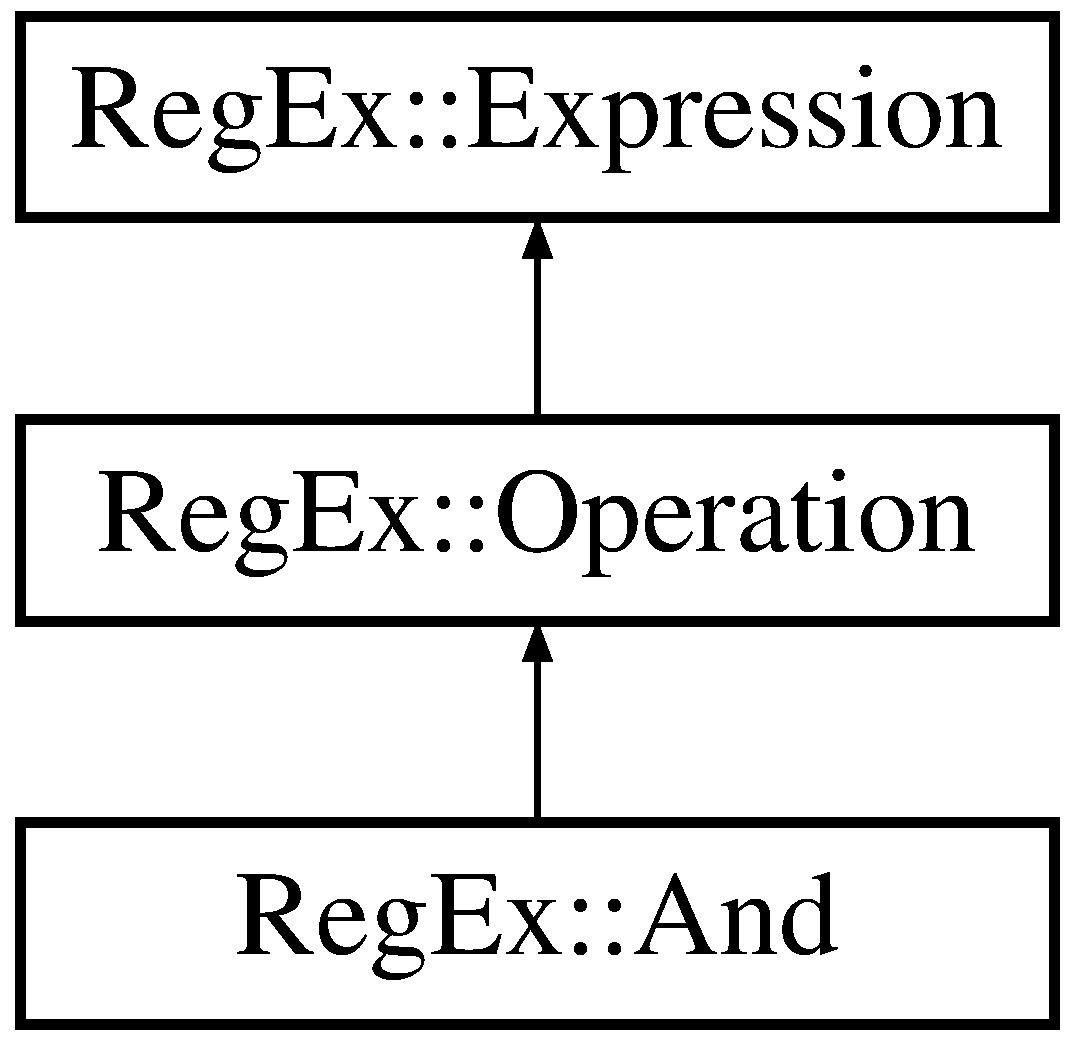
\includegraphics[height=3.000000cm]{class_reg_ex_1_1_and}
\end{center}
\end{figure}
\subsection*{Public Member Functions}
\begin{DoxyCompactItemize}
\item 
\mbox{\Hypertarget{class_reg_ex_1_1_and_a8810ebb2d7c45cef6246c4d019b18940}\label{class_reg_ex_1_1_and_a8810ebb2d7c45cef6246c4d019b18940}} 
{\bfseries And} (\hyperlink{class_reg_ex_1_1_expression}{Expression} $\ast$\+\_\+left\+\_\+exp, \hyperlink{class_reg_ex_1_1_expression}{Expression} $\ast$\+\_\+right\+\_\+exp)
\item 
\mbox{\Hypertarget{class_reg_ex_1_1_and_aeeb03347f3cf64d4313c49cf7df6edb8}\label{class_reg_ex_1_1_and_aeeb03347f3cf64d4313c49cf7df6edb8}} 
virtual void {\bfseries Generate} ()
\item 
\mbox{\Hypertarget{class_reg_ex_1_1_and_ae95a8c127ce73d9c595b7b3d9b63020d}\label{class_reg_ex_1_1_and_ae95a8c127ce73d9c595b7b3d9b63020d}} 
virtual std\+::string {\bfseries Get} ()
\end{DoxyCompactItemize}
\subsection*{Protected Attributes}
\begin{DoxyCompactItemize}
\item 
\mbox{\Hypertarget{class_reg_ex_1_1_and_ad523d9b208f99483a5f53471c32b6a37}\label{class_reg_ex_1_1_and_ad523d9b208f99483a5f53471c32b6a37}} 
\hyperlink{class_reg_ex_1_1_expression}{Expression} $\ast$ {\bfseries left\+\_\+exp\+\_\+}
\item 
\mbox{\Hypertarget{class_reg_ex_1_1_and_a0fa312b1550769293a5f68b1d05fb645}\label{class_reg_ex_1_1_and_a0fa312b1550769293a5f68b1d05fb645}} 
\hyperlink{class_reg_ex_1_1_expression}{Expression} $\ast$ {\bfseries right\+\_\+exp\+\_\+}
\end{DoxyCompactItemize}


The documentation for this class was generated from the following file\+:\begin{DoxyCompactItemize}
\item 
Reg\+Ex.\+h\end{DoxyCompactItemize}

\hypertarget{class_array}{}\section{Array Class Reference}
\label{class_array}\index{Array@{Array}}
Inheritance diagram for Array\+:\begin{figure}[H]
\begin{center}
\leavevmode
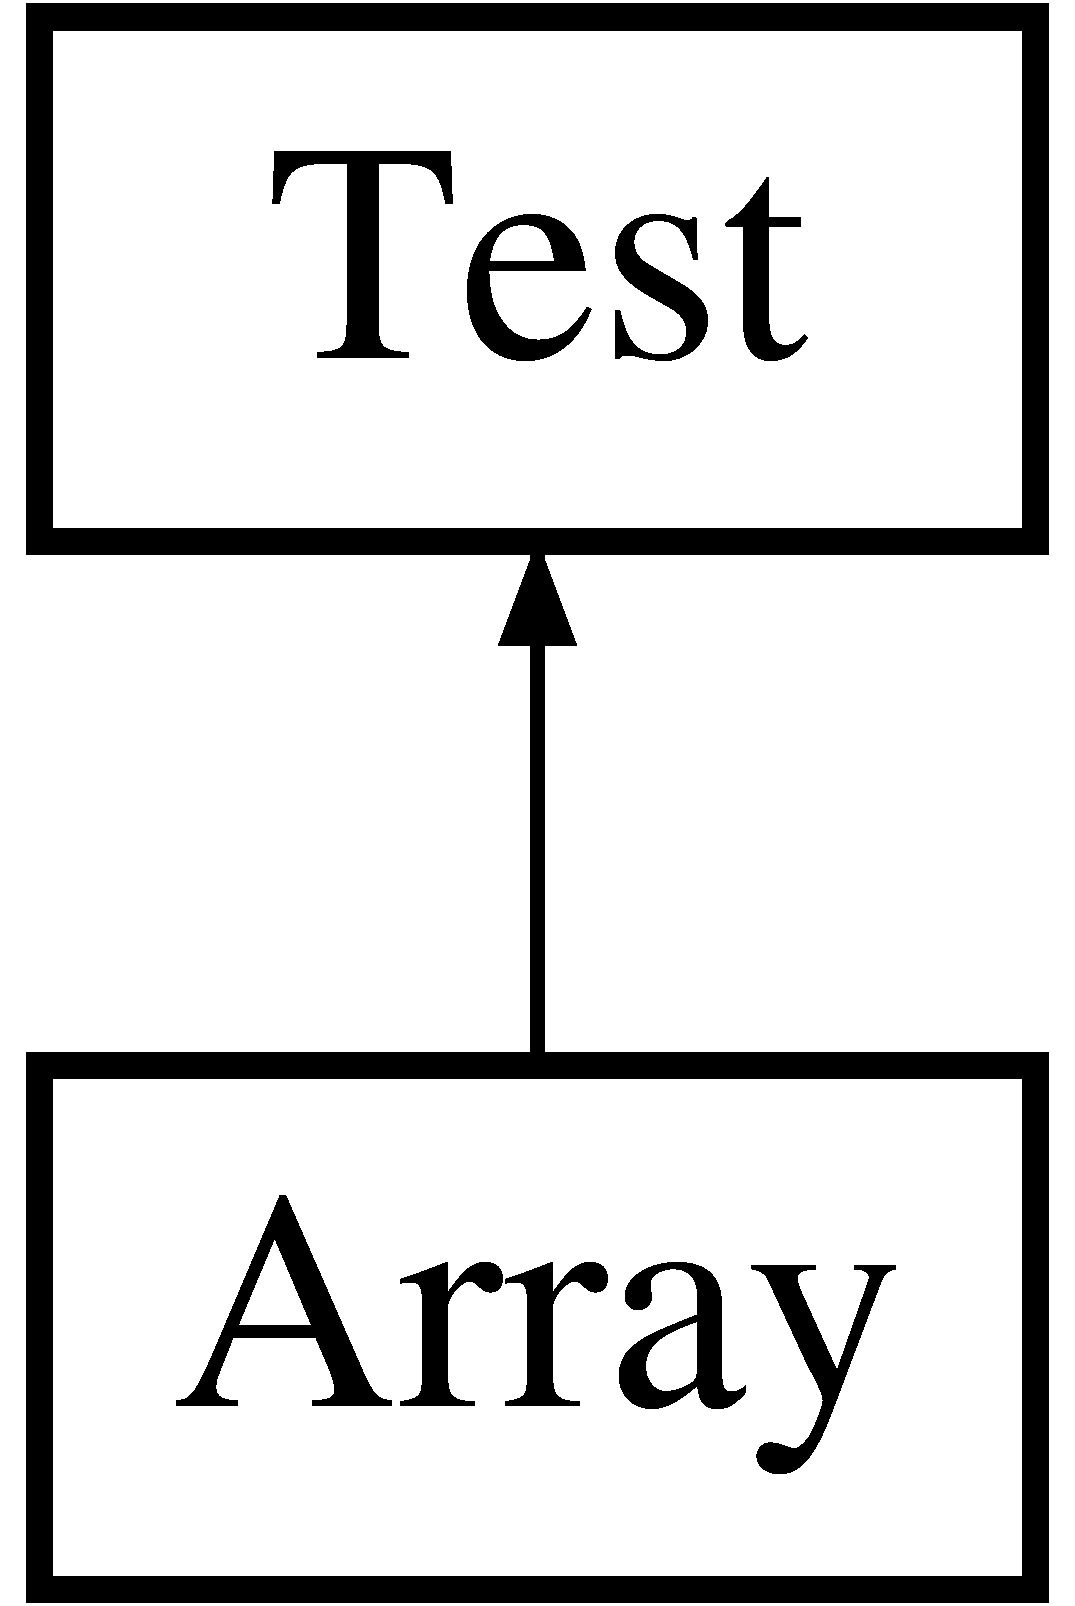
\includegraphics[height=2.000000cm]{class_array}
\end{center}
\end{figure}
\subsection*{Public Member Functions}
\begin{DoxyCompactItemize}
\item 
\mbox{\Hypertarget{class_array_aae39c85f40010b4a6697283edb6e09e6}\label{class_array_aae39c85f40010b4a6697283edb6e09e6}} 
{\bfseries Array} (\hyperlink{class_primitive_test}{Primitive\+Test}$<$ int $>$ $\ast$, std\+::function$<$ \hyperlink{class_test}{Test} $\ast$()$>$, std\+::string=\char`\"{} \char`\"{}, std\+::string=\char`\"{}\textbackslash{})
\item 
\mbox{\Hypertarget{class_array_a8afd0c475486567863069e3b20407de3}\label{class_array_a8afd0c475486567863069e3b20407de3}} 
{\bfseries Array} (\hyperlink{class_primitive_test}{Primitive\+Test}$<$ int $>$ $\ast$, \hyperlink{class_test}{Test} $\ast$, std\+::string=\char`\"{} \char`\"{}, std\+::string=\char`\"{}\textbackslash{})
\item 
\mbox{\Hypertarget{class_array_a8150dd2f8052651b58620712dab6b01d}\label{class_array_a8150dd2f8052651b58620712dab6b01d}} 
virtual void {\bfseries Generate} ()
\item 
\mbox{\Hypertarget{class_array_acd4f6a61bdf078fb95d88bfefde968b6}\label{class_array_acd4f6a61bdf078fb95d88bfefde968b6}} 
virtual void {\bfseries Print} (std\+::ostream \&=std\+::cout) const
\item 
\mbox{\Hypertarget{class_array_a00692e10c08fa00422f3c69dffaf493a}\label{class_array_a00692e10c08fa00422f3c69dffaf493a}} 
void {\bfseries Print\+Size} (bool)
\item 
\mbox{\Hypertarget{class_array_acd818a5c07a32f35f084e93db7459643}\label{class_array_acd818a5c07a32f35f084e93db7459643}} 
int {\bfseries Size} ()
\item 
\mbox{\Hypertarget{class_array_abc56765b098f851fbb87bf2210afb9db}\label{class_array_abc56765b098f851fbb87bf2210afb9db}} 
virtual \hyperlink{class_array}{Array} $\ast$ {\bfseries Clone} () const
\item 
\mbox{\Hypertarget{class_array_a52b6dbc5f68eea1434d70c66b7596a80}\label{class_array_a52b6dbc5f68eea1434d70c66b7596a80}} 
\hyperlink{class_test}{Test} $\ast$ {\bfseries operator\mbox{[}$\,$\mbox{]}} (int i)
\end{DoxyCompactItemize}
\subsection*{Protected Attributes}
\begin{DoxyCompactItemize}
\item 
\mbox{\Hypertarget{class_array_a575ef9a32841d1b1b56aa8ba7f8d5144}\label{class_array_a575ef9a32841d1b1b56aa8ba7f8d5144}} 
std\+::function$<$ \hyperlink{class_test}{Test} $\ast$()$>$ {\bfseries generation\+\_\+function\+\_\+}
\item 
\mbox{\Hypertarget{class_array_a43e6823f8b0acaf5c3b7599a9ab4d178}\label{class_array_a43e6823f8b0acaf5c3b7599a9ab4d178}} 
\hyperlink{class_test}{Test} $\ast$ {\bfseries example\+\_\+}
\item 
\mbox{\Hypertarget{class_array_afcafcb06168b848eeadd56c148e2d55f}\label{class_array_afcafcb06168b848eeadd56c148e2d55f}} 
\hyperlink{class_primitive_test}{Primitive\+Test}$<$ int $>$ $\ast$ {\bfseries array\+\_\+size\+\_\+}
\item 
\mbox{\Hypertarget{class_array_a08f0ba4ee6b95854dab20695506180a5}\label{class_array_a08f0ba4ee6b95854dab20695506180a5}} 
std\+::vector$<$ \hyperlink{class_test}{Test} $\ast$ $>$ {\bfseries array\+\_\+}
\item 
\mbox{\Hypertarget{class_array_ab7f48d91eb1c9747cb7b7aaddf13cb20}\label{class_array_ab7f48d91eb1c9747cb7b7aaddf13cb20}} 
std\+::string {\bfseries delimiter\+\_\+}
\item 
\mbox{\Hypertarget{class_array_a4012ececf0120797b633f8be52b5b929}\label{class_array_a4012ececf0120797b633f8be52b5b929}} 
std\+::string {\bfseries line\+\_\+breaker\+\_\+}
\item 
\mbox{\Hypertarget{class_array_a71aba3c107c87e27ae66e9a9a703c2b2}\label{class_array_a71aba3c107c87e27ae66e9a9a703c2b2}} 
bool {\bfseries print\+\_\+size\+\_\+}
\end{DoxyCompactItemize}


The documentation for this class was generated from the following files\+:\begin{DoxyCompactItemize}
\item 
Array.\+h\item 
Array.\+cpp\end{DoxyCompactItemize}

\hypertarget{class_b_g}{}\section{BG Class Reference}
\label{class_b_g}\index{BG@{BG}}
Inheritance diagram for BG\+:\begin{figure}[H]
\begin{center}
\leavevmode
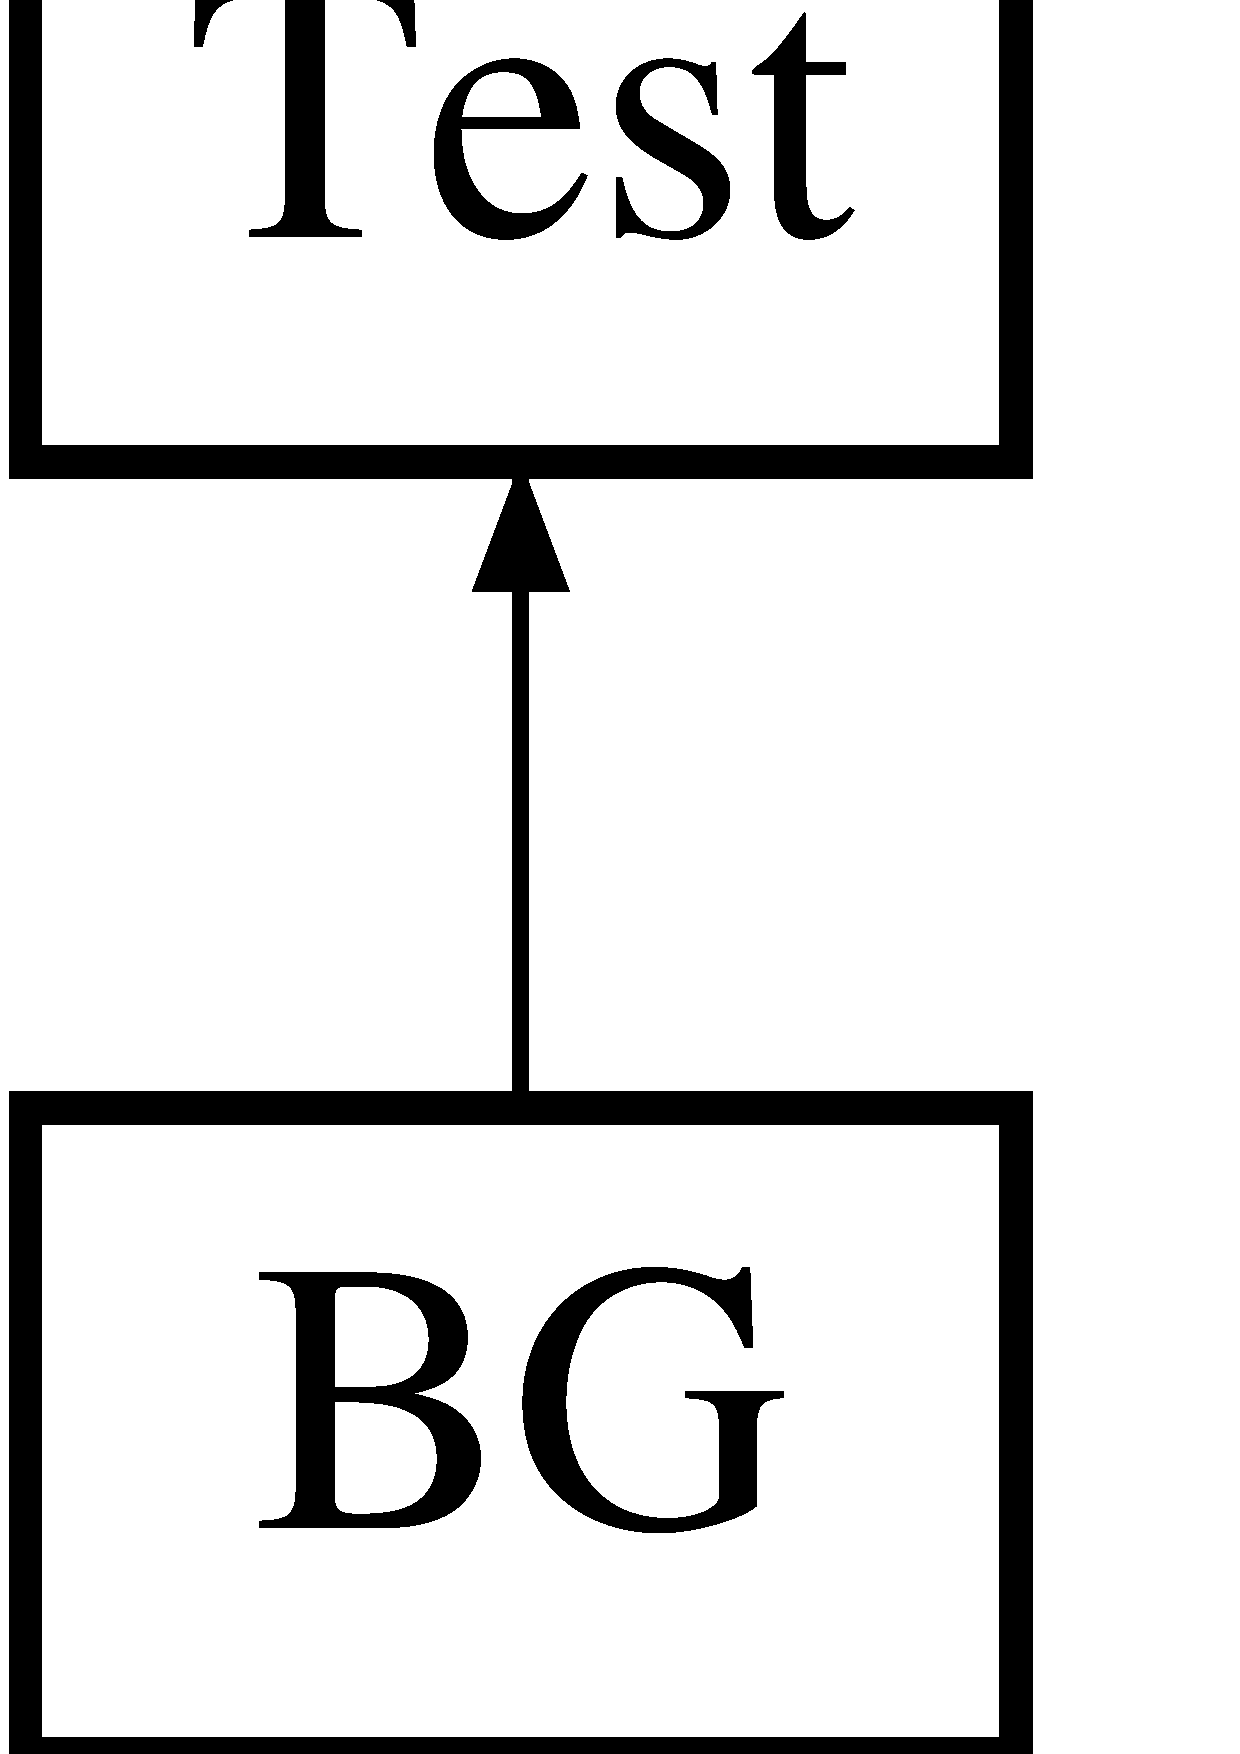
\includegraphics[height=2.000000cm]{class_b_g}
\end{center}
\end{figure}
\subsection*{Public Member Functions}
\begin{DoxyCompactItemize}
\item 
\mbox{\Hypertarget{class_b_g_a8f4a9870c4f6cd7f27160200f2f7560b}\label{class_b_g_a8f4a9870c4f6cd7f27160200f2f7560b}} 
virtual void {\bfseries Generate} ()
\item 
\mbox{\Hypertarget{class_b_g_aff8adc384fc9aef8d689e640ba66f073}\label{class_b_g_aff8adc384fc9aef8d689e640ba66f073}} 
virtual void {\bfseries Print} (std\+::ostream \&\+\_\+out) const
\item 
\mbox{\Hypertarget{class_b_g_a4ab2348538cec6d125e3d5e7872f32ff}\label{class_b_g_a4ab2348538cec6d125e3d5e7872f32ff}} 
virtual \hyperlink{class_test}{Test} $\ast$ {\bfseries Clone} () const
\end{DoxyCompactItemize}
\subsection*{Additional Inherited Members}


The documentation for this class was generated from the following file\+:\begin{DoxyCompactItemize}
\item 
Source.\+cpp\end{DoxyCompactItemize}

\hypertarget{class_binary_tree}{}\section{Binary\+Tree Class Reference}
\label{class_binary_tree}\index{Binary\+Tree@{Binary\+Tree}}
Inheritance diagram for Binary\+Tree\+:\begin{figure}[H]
\begin{center}
\leavevmode
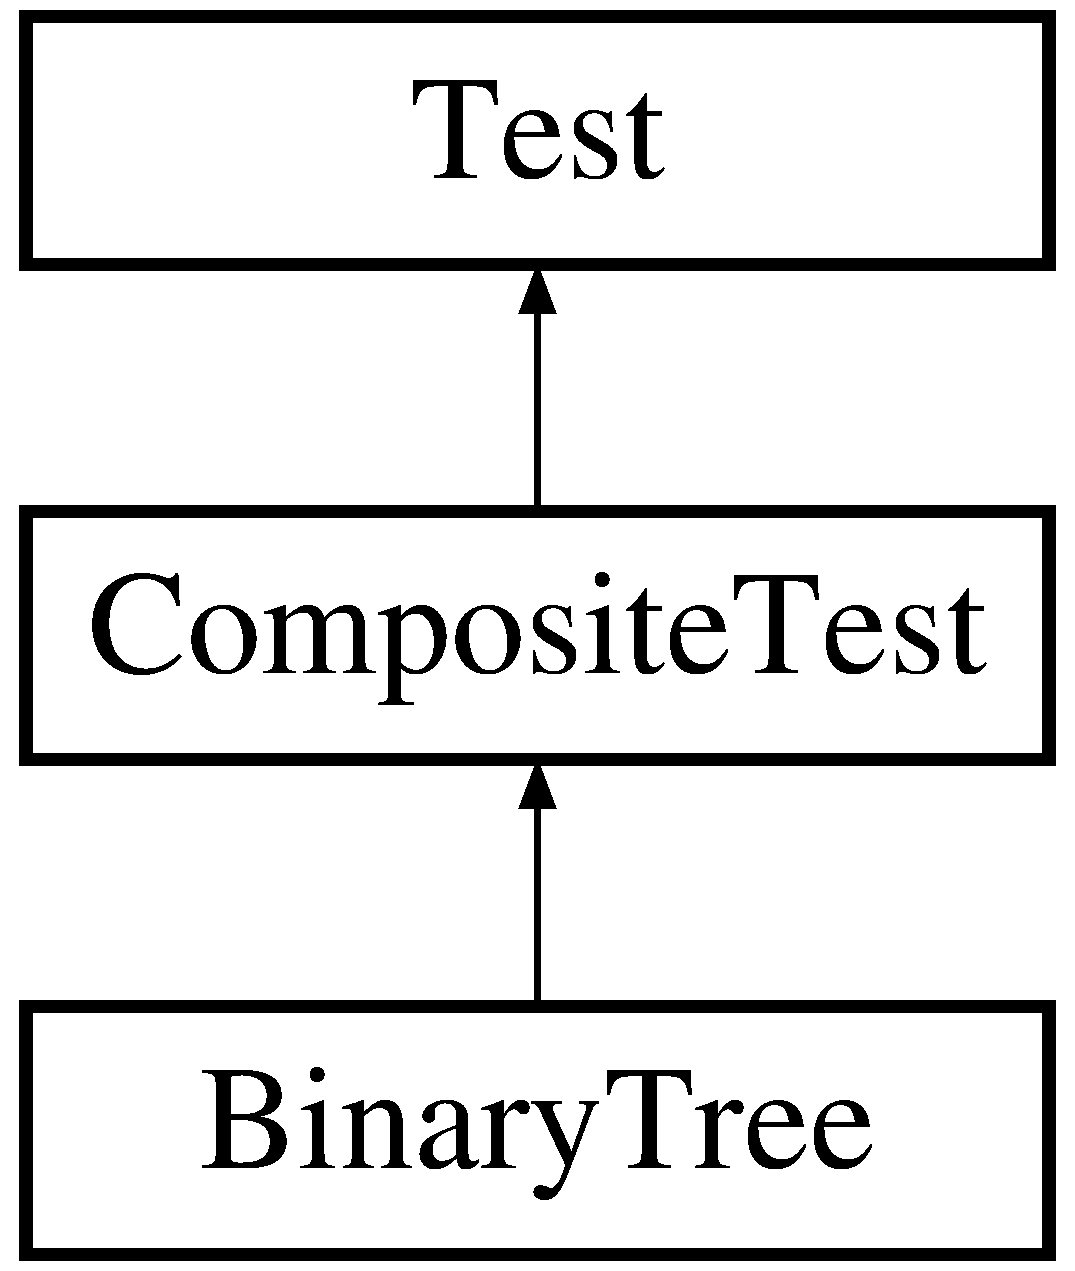
\includegraphics[height=3.000000cm]{class_binary_tree}
\end{center}
\end{figure}
\subsection*{Public Member Functions}
\begin{DoxyCompactItemize}
\item 
\mbox{\Hypertarget{class_binary_tree_a115788642169d3b9e8cccc8456a59091}\label{class_binary_tree_a115788642169d3b9e8cccc8456a59091}} 
{\bfseries Binary\+Tree} (int \+\_\+depth)
\item 
\mbox{\Hypertarget{class_binary_tree_a5797bee232ef3dc202c8fa6a54613806}\label{class_binary_tree_a5797bee232ef3dc202c8fa6a54613806}} 
void {\bfseries E} ()
\item 
\mbox{\Hypertarget{class_binary_tree_a3c3b9ca7202c16f17259740a4b4a359c}\label{class_binary_tree_a3c3b9ca7202c16f17259740a4b4a359c}} 
void {\bfseries Generate} ()
\end{DoxyCompactItemize}
\subsection*{Additional Inherited Members}


The documentation for this class was generated from the following file\+:\begin{DoxyCompactItemize}
\item 
Source.\+cpp\end{DoxyCompactItemize}

\hypertarget{class_composite_test}{}\section{Composite\+Test Class Reference}
\label{class_composite_test}\index{Composite\+Test@{Composite\+Test}}
Inheritance diagram for Composite\+Test\+:\begin{figure}[H]
\begin{center}
\leavevmode
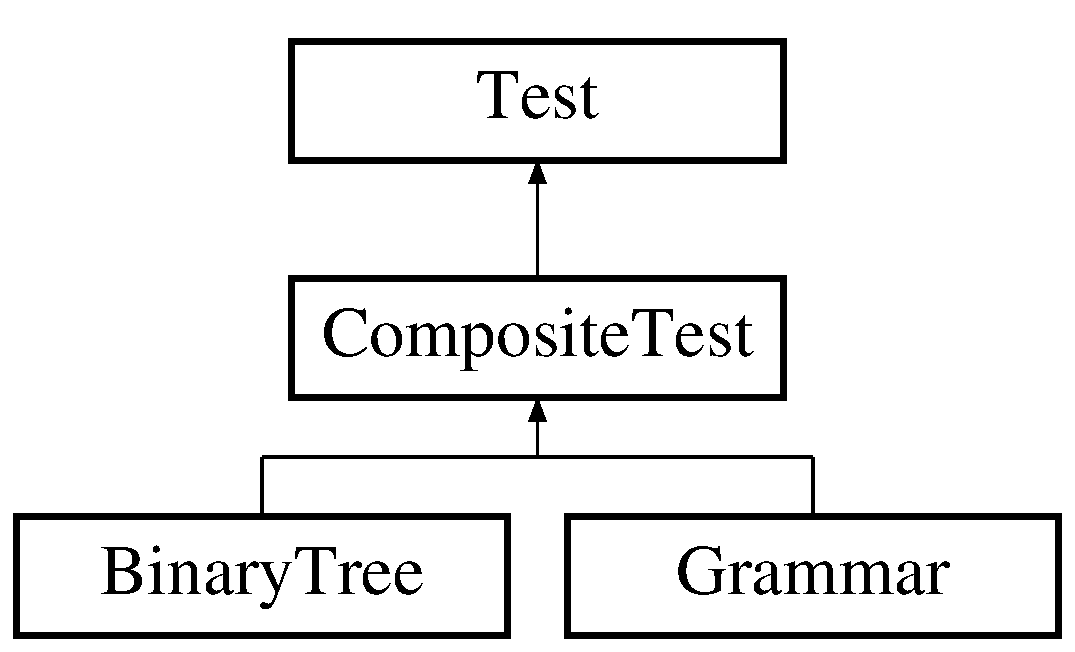
\includegraphics[height=3.000000cm]{class_composite_test}
\end{center}
\end{figure}
\subsection*{Public Member Functions}
\begin{DoxyCompactItemize}
\item 
\mbox{\Hypertarget{class_composite_test_ad0e6a5fd6360ce96743c636d717a233d}\label{class_composite_test_ad0e6a5fd6360ce96743c636d717a233d}} 
virtual \hyperlink{class_test}{Test} $\ast$ {\bfseries Add} (\hyperlink{class_test}{Test} $\ast$)
\item 
\mbox{\Hypertarget{class_composite_test_abfb08ce280fe059e6cf738ba0fadc9e3}\label{class_composite_test_abfb08ce280fe059e6cf738ba0fadc9e3}} 
virtual void {\bfseries Clear} ()
\item 
\mbox{\Hypertarget{class_composite_test_a09cc295cd80dc282b67dbdd4c6b61ae6}\label{class_composite_test_a09cc295cd80dc282b67dbdd4c6b61ae6}} 
virtual void {\bfseries Generate} ()
\item 
\mbox{\Hypertarget{class_composite_test_a24dec1bf9fdb38b7d58c3a7049342db3}\label{class_composite_test_a24dec1bf9fdb38b7d58c3a7049342db3}} 
virtual void {\bfseries Print} (std\+::ostream \&=std\+::cout) const
\item 
\mbox{\Hypertarget{class_composite_test_aa145bb15f0f6b3a18ac6b1abf2e4e4b9}\label{class_composite_test_aa145bb15f0f6b3a18ac6b1abf2e4e4b9}} 
virtual \hyperlink{class_composite_test}{Composite\+Test} $\ast$ {\bfseries Clone} () const
\end{DoxyCompactItemize}
\subsection*{Protected Attributes}
\begin{DoxyCompactItemize}
\item 
\mbox{\Hypertarget{class_composite_test_a9c48b83daaec8de1a28aa813b7ee150e}\label{class_composite_test_a9c48b83daaec8de1a28aa813b7ee150e}} 
std\+::vector$<$ \hyperlink{class_test}{Test} $\ast$ $>$ {\bfseries tests\+\_\+}
\end{DoxyCompactItemize}


The documentation for this class was generated from the following files\+:\begin{DoxyCompactItemize}
\item 
Composite\+Test.\+h\item 
Composite\+Test.\+cpp\end{DoxyCompactItemize}

\hypertarget{class_const_primitive_test}{}\section{Const\+Primitive\+Test$<$ T $>$ Class Template Reference}
\label{class_const_primitive_test}\index{Const\+Primitive\+Test$<$ T $>$@{Const\+Primitive\+Test$<$ T $>$}}
Inheritance diagram for Const\+Primitive\+Test$<$ T $>$\+:\begin{figure}[H]
\begin{center}
\leavevmode
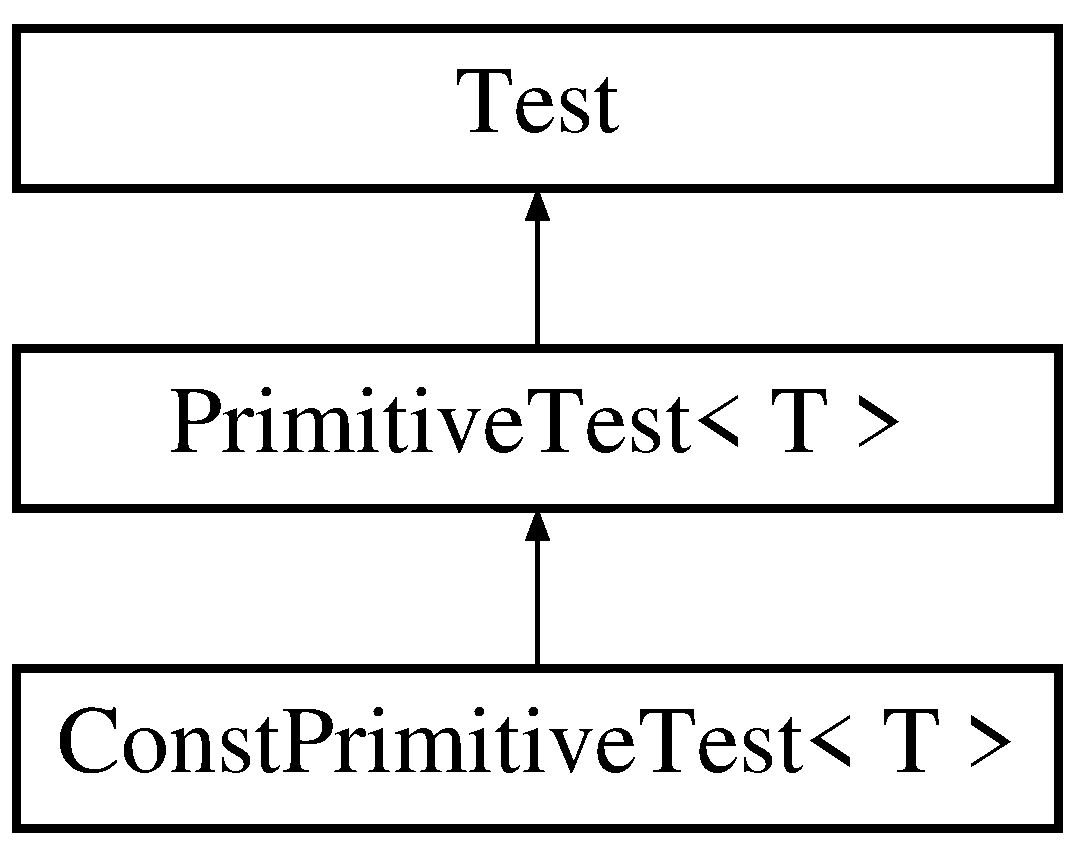
\includegraphics[height=3.000000cm]{class_const_primitive_test}
\end{center}
\end{figure}
\subsection*{Public Member Functions}
\begin{DoxyCompactItemize}
\item 
\mbox{\Hypertarget{class_const_primitive_test_a34da605f489cab8f071ac3130916e67f}\label{class_const_primitive_test_a34da605f489cab8f071ac3130916e67f}} 
{\bfseries Const\+Primitive\+Test} (T \+\_\+value=0)
\item 
\mbox{\Hypertarget{class_const_primitive_test_a081b3449770c6d020bd1116e8ffdb293}\label{class_const_primitive_test_a081b3449770c6d020bd1116e8ffdb293}} 
virtual T {\bfseries Get} ()
\item 
\mbox{\Hypertarget{class_const_primitive_test_a121caecc26a0a3fb1ba72c5590ce2cf3}\label{class_const_primitive_test_a121caecc26a0a3fb1ba72c5590ce2cf3}} 
virtual void {\bfseries Generate} ()
\item 
\mbox{\Hypertarget{class_const_primitive_test_af9e8401d681d647cab2f154838bc387c}\label{class_const_primitive_test_af9e8401d681d647cab2f154838bc387c}} 
virtual void {\bfseries Print} (std\+::ostream \&\+\_\+out=std\+::cout) const
\item 
\mbox{\Hypertarget{class_const_primitive_test_a31b6a7a42f6e3677a71b1c9017ddb348}\label{class_const_primitive_test_a31b6a7a42f6e3677a71b1c9017ddb348}} 
virtual \hyperlink{class_const_primitive_test}{Const\+Primitive\+Test} $\ast$ {\bfseries Clone} () const
\item 
\mbox{\Hypertarget{class_const_primitive_test_a5b834edb4d45951d0ea3d95238328c04}\label{class_const_primitive_test_a5b834edb4d45951d0ea3d95238328c04}} 
\hyperlink{class_const_primitive_test}{Const\+Primitive\+Test}$<$ T $>$ \& {\bfseries operator=} (T \+\_\+current\+\_\+value)
\end{DoxyCompactItemize}
\subsection*{Protected Attributes}
\begin{DoxyCompactItemize}
\item 
\mbox{\Hypertarget{class_const_primitive_test_a63135178fde91f8b9dc557255d8cce85}\label{class_const_primitive_test_a63135178fde91f8b9dc557255d8cce85}} 
T {\bfseries current\+\_\+value\+\_\+}
\end{DoxyCompactItemize}


The documentation for this class was generated from the following file\+:\begin{DoxyCompactItemize}
\item 
Const\+Primitive\+Test.\+h\end{DoxyCompactItemize}

\hypertarget{class_const_string_set}{}\section{Const\+String\+Set Class Reference}
\label{class_const_string_set}\index{Const\+String\+Set@{Const\+String\+Set}}
Inheritance diagram for Const\+String\+Set\+:\begin{figure}[H]
\begin{center}
\leavevmode
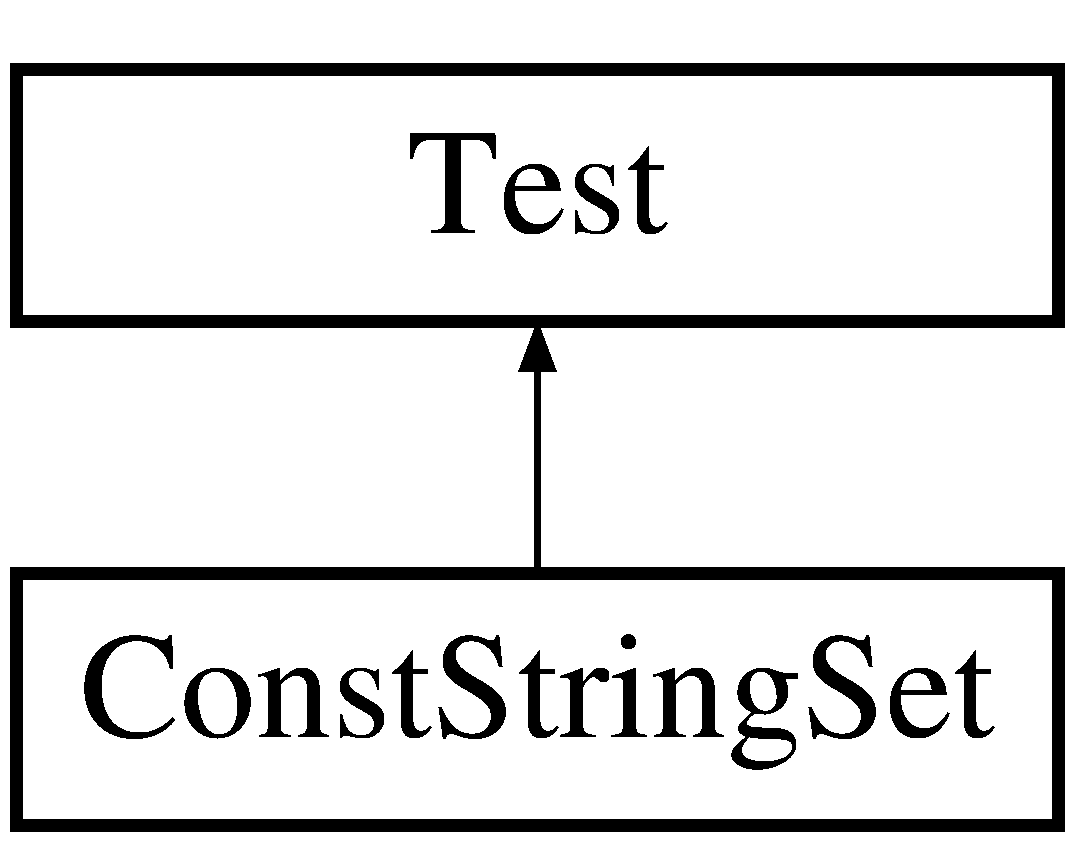
\includegraphics[height=2.000000cm]{class_const_string_set}
\end{center}
\end{figure}
\subsection*{Public Member Functions}
\begin{DoxyCompactItemize}
\item 
\mbox{\Hypertarget{class_const_string_set_acd0a1079f684d1c210738414ed6ba61d}\label{class_const_string_set_acd0a1079f684d1c210738414ed6ba61d}} 
virtual \hyperlink{class_const_string_set}{Const\+String\+Set} $\ast$ {\bfseries Add} (std\+::string)
\item 
\mbox{\Hypertarget{class_const_string_set_ae4ab97db08d0aaf52a04e3927941cb5d}\label{class_const_string_set_ae4ab97db08d0aaf52a04e3927941cb5d}} 
virtual \hyperlink{class_const_string_set}{Const\+String\+Set} $\ast$ {\bfseries Add} (char)
\item 
\mbox{\Hypertarget{class_const_string_set_a817a9530b8107ed97250c539d74c5f52}\label{class_const_string_set_a817a9530b8107ed97250c539d74c5f52}} 
virtual std\+::string {\bfseries Get} ()
\item 
\mbox{\Hypertarget{class_const_string_set_a5f1fdb968a310f7e7a15295ae05388d4}\label{class_const_string_set_a5f1fdb968a310f7e7a15295ae05388d4}} 
virtual void {\bfseries Generate} ()
\item 
\mbox{\Hypertarget{class_const_string_set_a60612742de31f7556c76dd5306e5af92}\label{class_const_string_set_a60612742de31f7556c76dd5306e5af92}} 
virtual void {\bfseries Print} (std\+::ostream \&=std\+::cout) const
\item 
\mbox{\Hypertarget{class_const_string_set_aba9c7cefc8063c338241f52feb007403}\label{class_const_string_set_aba9c7cefc8063c338241f52feb007403}} 
virtual \hyperlink{class_const_string_set}{Const\+String\+Set} $\ast$ {\bfseries Clone} () const
\end{DoxyCompactItemize}
\subsection*{Protected Attributes}
\begin{DoxyCompactItemize}
\item 
\mbox{\Hypertarget{class_const_string_set_a10df2e2eb9996b186a5ebc5eb5bb39ff}\label{class_const_string_set_a10df2e2eb9996b186a5ebc5eb5bb39ff}} 
std\+::set$<$ std\+::string $>$ {\bfseries set\+\_\+}
\item 
\mbox{\Hypertarget{class_const_string_set_a44b41982c0af8089d6305d1b7182e3ce}\label{class_const_string_set_a44b41982c0af8089d6305d1b7182e3ce}} 
std\+::vector$<$ std\+::string $>$ {\bfseries elements}
\item 
\mbox{\Hypertarget{class_const_string_set_aaf3ae758c73013b2969da9db406d017f}\label{class_const_string_set_aaf3ae758c73013b2969da9db406d017f}} 
std\+::string {\bfseries current\+\_\+string\+\_\+}
\end{DoxyCompactItemize}


The documentation for this class was generated from the following files\+:\begin{DoxyCompactItemize}
\item 
Const\+String\+Set.\+h\item 
Const\+String\+Set.\+cpp\end{DoxyCompactItemize}

\hypertarget{class_delimiter}{}\section{Delimiter Class Reference}
\label{class_delimiter}\index{Delimiter@{Delimiter}}
Inheritance diagram for Delimiter\+:\begin{figure}[H]
\begin{center}
\leavevmode
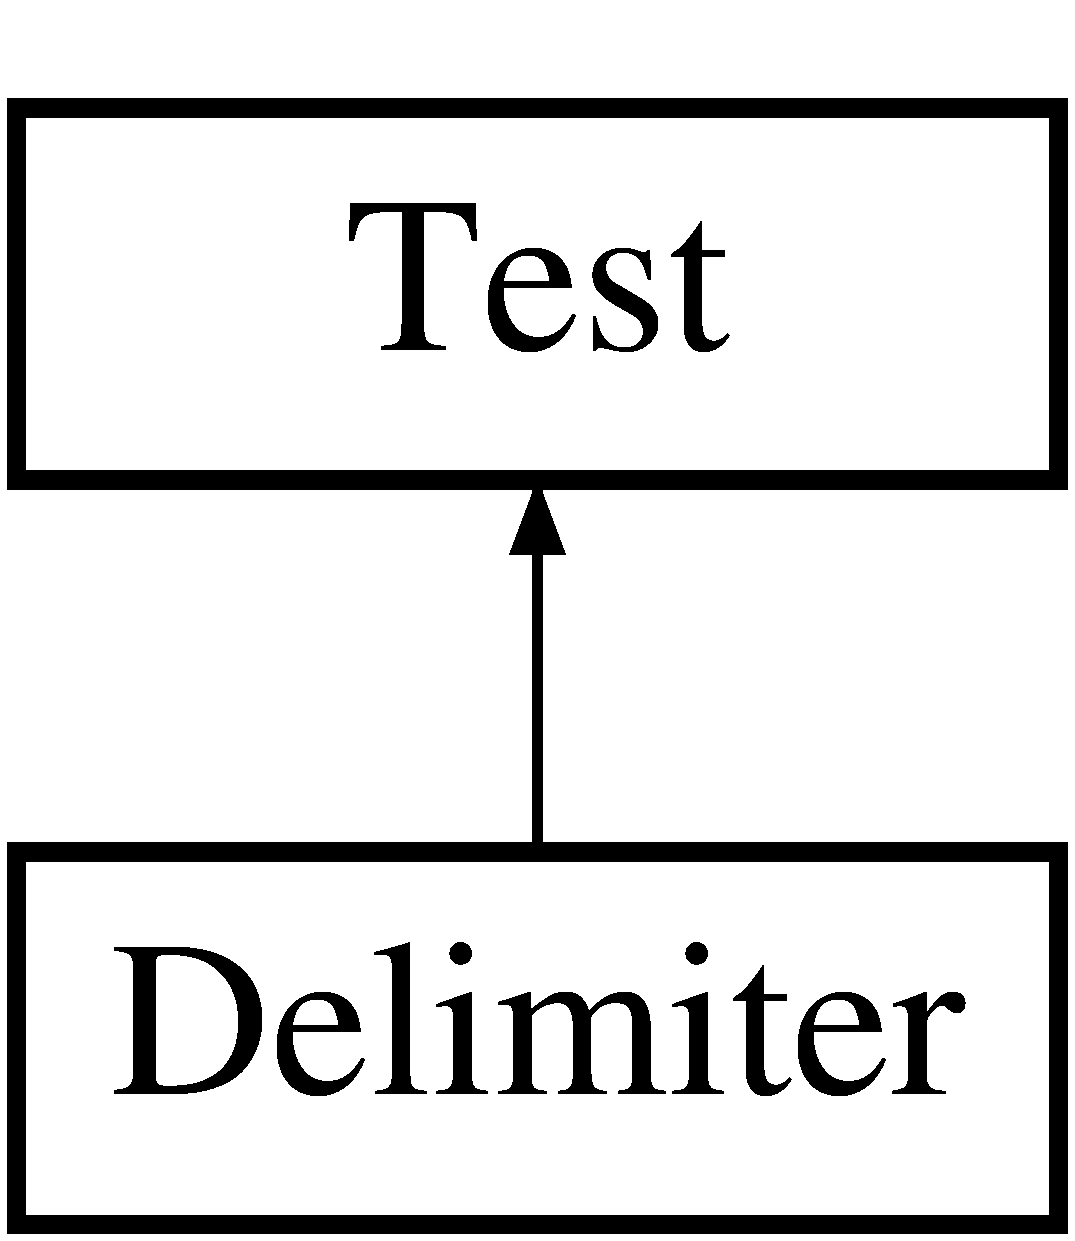
\includegraphics[height=2.000000cm]{class_delimiter}
\end{center}
\end{figure}
\subsection*{Public Member Functions}
\begin{DoxyCompactItemize}
\item 
\mbox{\Hypertarget{class_delimiter_a3f71d4befe98c343885843020d73fe57}\label{class_delimiter_a3f71d4befe98c343885843020d73fe57}} 
{\bfseries Delimiter} (char)
\item 
\mbox{\Hypertarget{class_delimiter_a7f8b3d11a61da117b16266698e3970f9}\label{class_delimiter_a7f8b3d11a61da117b16266698e3970f9}} 
{\bfseries Delimiter} (std\+::string)
\item 
\mbox{\Hypertarget{class_delimiter_a41243428a72c32819ac06054eceb1849}\label{class_delimiter_a41243428a72c32819ac06054eceb1849}} 
std\+::string {\bfseries Get} ()
\item 
\mbox{\Hypertarget{class_delimiter_a97018f86a44c47accc7159005b6a8c51}\label{class_delimiter_a97018f86a44c47accc7159005b6a8c51}} 
virtual void {\bfseries Generate} ()
\item 
\mbox{\Hypertarget{class_delimiter_acb6a47271dbe1bda372e1a80bcfad31b}\label{class_delimiter_acb6a47271dbe1bda372e1a80bcfad31b}} 
virtual void {\bfseries Print} (std\+::ostream \&=std\+::cout) const
\item 
\mbox{\Hypertarget{class_delimiter_a50030fab46791d71fe369bada8bd2b89}\label{class_delimiter_a50030fab46791d71fe369bada8bd2b89}} 
virtual \hyperlink{class_delimiter}{Delimiter} $\ast$ {\bfseries Clone} () const
\end{DoxyCompactItemize}
\subsection*{Protected Attributes}
\begin{DoxyCompactItemize}
\item 
\mbox{\Hypertarget{class_delimiter_a84e0f61d961047ae5badb99a132ddfc2}\label{class_delimiter_a84e0f61d961047ae5badb99a132ddfc2}} 
std\+::string {\bfseries delimiter\+\_\+}
\end{DoxyCompactItemize}


The documentation for this class was generated from the following files\+:\begin{DoxyCompactItemize}
\item 
Delimiter.\+h\item 
Delimiter.\+cpp\end{DoxyCompactItemize}

\hypertarget{class_reg_ex_1_1_expression}{}\section{Reg\+Ex\+:\+:Expression Class Reference}
\label{class_reg_ex_1_1_expression}\index{Reg\+Ex\+::\+Expression@{Reg\+Ex\+::\+Expression}}
Inheritance diagram for Reg\+Ex\+:\+:Expression\+:\begin{figure}[H]
\begin{center}
\leavevmode
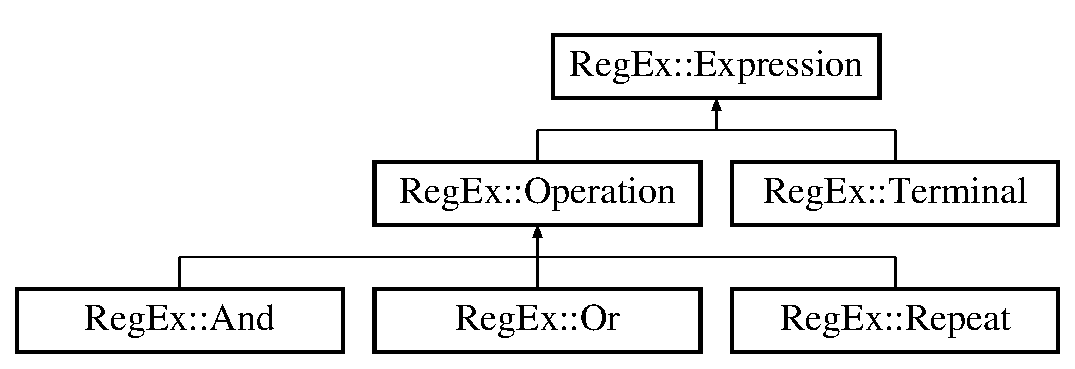
\includegraphics[height=3.000000cm]{class_reg_ex_1_1_expression}
\end{center}
\end{figure}
\subsection*{Public Member Functions}
\begin{DoxyCompactItemize}
\item 
\mbox{\Hypertarget{class_reg_ex_1_1_expression_a77ab5c127ba289ba3071134161d3d8f9}\label{class_reg_ex_1_1_expression_a77ab5c127ba289ba3071134161d3d8f9}} 
virtual void {\bfseries Generate} ()=0
\item 
\mbox{\Hypertarget{class_reg_ex_1_1_expression_a204f8b3b433b1ed46de48688dcedc140}\label{class_reg_ex_1_1_expression_a204f8b3b433b1ed46de48688dcedc140}} 
virtual std\+::string {\bfseries Get} ()=0
\end{DoxyCompactItemize}


The documentation for this class was generated from the following file\+:\begin{DoxyCompactItemize}
\item 
Reg\+Ex.\+h\end{DoxyCompactItemize}

\hypertarget{class_grammar}{}\section{Grammar Class Reference}
\label{class_grammar}\index{Grammar@{Grammar}}
Inheritance diagram for Grammar\+:\begin{figure}[H]
\begin{center}
\leavevmode
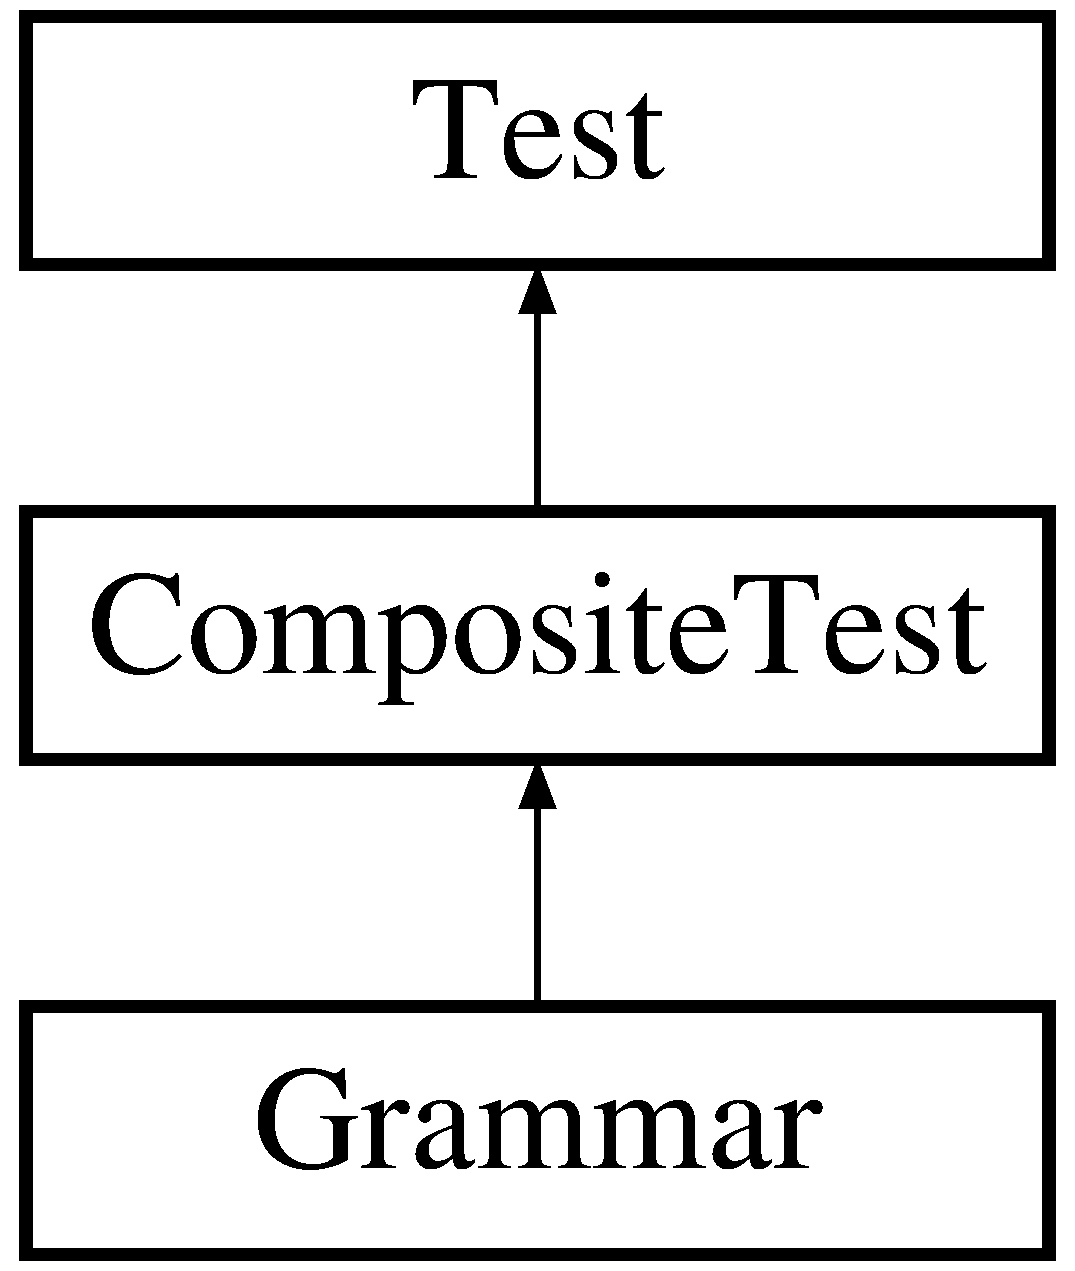
\includegraphics[height=3.000000cm]{class_grammar}
\end{center}
\end{figure}
\subsection*{Public Member Functions}
\begin{DoxyCompactItemize}
\item 
\mbox{\Hypertarget{class_grammar_a5ae4e5db880c0167b6d70934308ecdf7}\label{class_grammar_a5ae4e5db880c0167b6d70934308ecdf7}} 
{\bfseries Grammar} (const std\+::string \&, const std\+::string \&)
\item 
\mbox{\Hypertarget{class_grammar_aa3769b85b2ca3eba1d0af9cd77aa9b9d}\label{class_grammar_aa3769b85b2ca3eba1d0af9cd77aa9b9d}} 
virtual void {\bfseries Generator} (const std\+::string \&)
\item 
\mbox{\Hypertarget{class_grammar_a186953ca011692489432971cec4965f7}\label{class_grammar_a186953ca011692489432971cec4965f7}} 
virtual void {\bfseries Generate} ()
\item 
\mbox{\Hypertarget{class_grammar_a79f12115faf53b231e34b1e40e443664}\label{class_grammar_a79f12115faf53b231e34b1e40e443664}} 
virtual void {\bfseries Non\+Terms\+Parsing} (const std\+::string \&)
\item 
\mbox{\Hypertarget{class_grammar_a782f41eac47978d515b4ba5fa06c37dd}\label{class_grammar_a782f41eac47978d515b4ba5fa06c37dd}} 
virtual void {\bfseries Start\+Non\+Term\+Parsing} (const std\+::string \&)
\item 
\mbox{\Hypertarget{class_grammar_a119ada593ad12ff9940a49eb1f71c9f4}\label{class_grammar_a119ada593ad12ff9940a49eb1f71c9f4}} 
virtual void {\bfseries Terms\+Parsing} (const std\+::string \&)
\item 
\mbox{\Hypertarget{class_grammar_a251593d0e88bd99a1c8f55b065f4d39b}\label{class_grammar_a251593d0e88bd99a1c8f55b065f4d39b}} 
virtual void {\bfseries Rule\+Parsing} (const std\+::string \&)
\item 
\mbox{\Hypertarget{class_grammar_aaf6ab2ee1f6988426f6796c12451e208}\label{class_grammar_aaf6ab2ee1f6988426f6796c12451e208}} 
virtual void {\bfseries Grammar\+Parsing} ()
\item 
\mbox{\Hypertarget{class_grammar_a88135fd39f2bac99c761b1feef9d8c00}\label{class_grammar_a88135fd39f2bac99c761b1feef9d8c00}} 
virtual void {\bfseries Print} (std\+::ostream \&=std\+::cout) const
\item 
\mbox{\Hypertarget{class_grammar_aecd99c02c9e13da44969cd9b07db7dcc}\label{class_grammar_aecd99c02c9e13da44969cd9b07db7dcc}} 
virtual \hyperlink{class_grammar}{Grammar} $\ast$ {\bfseries Clone} () const
\end{DoxyCompactItemize}
\subsection*{Protected Attributes}
\begin{DoxyCompactItemize}
\item 
\mbox{\Hypertarget{class_grammar_ad48a06416c658caaab2c6a7d6c538bd9}\label{class_grammar_ad48a06416c658caaab2c6a7d6c538bd9}} 
std\+::string {\bfseries grammar\+\_\+}
\item 
\mbox{\Hypertarget{class_grammar_a660a540727807dfd9c3152b245377544}\label{class_grammar_a660a540727807dfd9c3152b245377544}} 
std\+::string {\bfseries rules\+\_\+}
\item 
\mbox{\Hypertarget{class_grammar_a124b3128fe6b0df7845a5e9fefb1f530}\label{class_grammar_a124b3128fe6b0df7845a5e9fefb1f530}} 
std\+::map$<$ std\+::string, std\+::vector$<$ std\+::string $>$ $>$ {\bfseries parsed\+\_\+rules\+\_\+}
\item 
\mbox{\Hypertarget{class_grammar_a4f20c5e5df17ca2c5ad53aaec4240b0b}\label{class_grammar_a4f20c5e5df17ca2c5ad53aaec4240b0b}} 
std\+::set$<$ std\+::string $>$ {\bfseries names\+\_\+of\+\_\+nonterm\+\_\+}
\item 
\mbox{\Hypertarget{class_grammar_a7664c4481949296f8a706de7049a6cf2}\label{class_grammar_a7664c4481949296f8a706de7049a6cf2}} 
std\+::set$<$ char $>$ {\bfseries terms\+\_\+}
\item 
\mbox{\Hypertarget{class_grammar_af02a912c7e3b2fa19049bf7fb3f4b815}\label{class_grammar_af02a912c7e3b2fa19049bf7fb3f4b815}} 
std\+::string {\bfseries start\+\_\+nonterm\+\_\+}
\item 
\mbox{\Hypertarget{class_grammar_a1be4add6568bdc37256a7affba21fbca}\label{class_grammar_a1be4add6568bdc37256a7affba21fbca}} 
std\+::string {\bfseries current\+\_\+string\+\_\+}
\end{DoxyCompactItemize}


The documentation for this class was generated from the following files\+:\begin{DoxyCompactItemize}
\item 
Grammar.\+h\item 
Grammar.\+cpp\end{DoxyCompactItemize}

\hypertarget{class_graph}{}\section{Graph Class Reference}
\label{class_graph}\index{Graph@{Graph}}
Inheritance diagram for Graph\+:\begin{figure}[H]
\begin{center}
\leavevmode
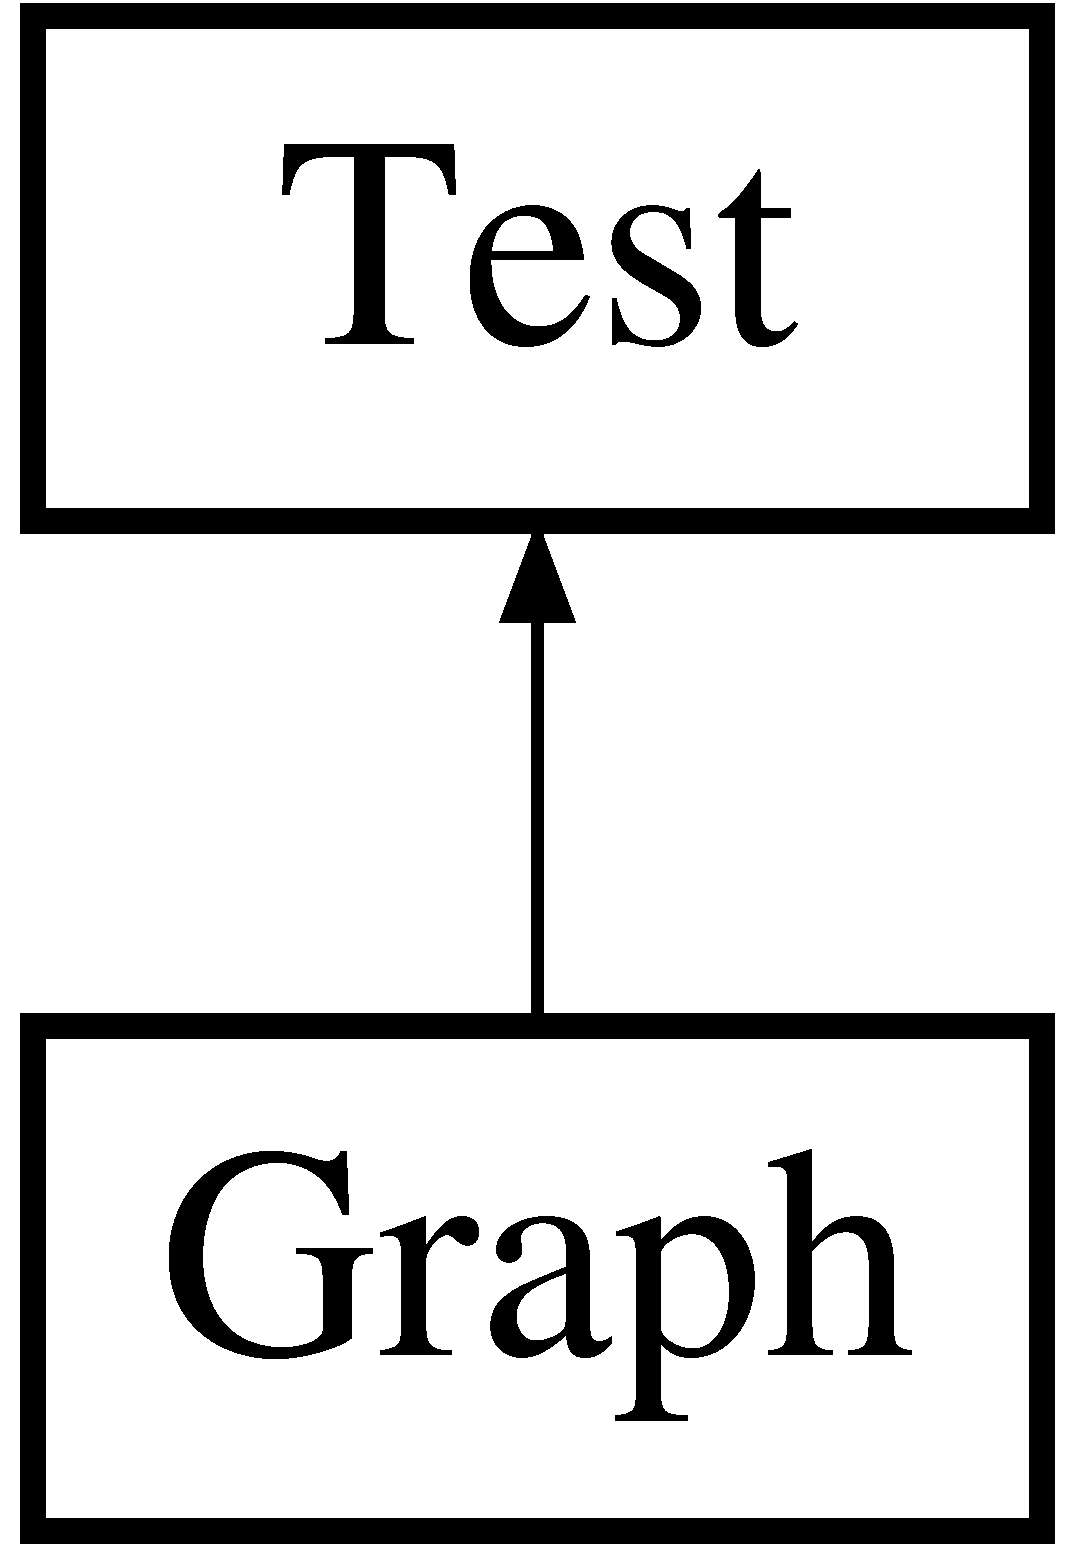
\includegraphics[height=2.000000cm]{class_graph}
\end{center}
\end{figure}
\subsection*{Public Types}
\begin{DoxyCompactItemize}
\item 
\mbox{\Hypertarget{class_graph_aabbabd0059aba1f53232d846cd7ca39e}\label{class_graph_aabbabd0059aba1f53232d846cd7ca39e}} 
enum {\bfseries P\+R\+I\+N\+T\+\_\+\+T\+Y\+PE} \{ {\bfseries C\+O\+N\+N\+E\+C\+T\+I\+O\+N\+\_\+\+M\+A\+T\+R\+IX}, 
{\bfseries C\+O\+N\+N\+E\+C\+T\+I\+O\+N\+\_\+\+L\+I\+ST}, 
{\bfseries L\+I\+S\+T\+\_\+\+O\+F\+\_\+\+E\+D\+G\+ES}
 \}
\end{DoxyCompactItemize}
\subsection*{Public Member Functions}
\begin{DoxyCompactItemize}
\item 
\hyperlink{class_graph_a480d475b69a6b892b044b255a5fb47f5}{Graph} (\hyperlink{class_primitive_test}{Primitive\+Test}$<$ int $>$ $\ast$\+\_\+number\+\_\+of\+\_\+vertices, \hyperlink{class_primitive_test}{Primitive\+Test}$<$ int $>$ $\ast$\+\_\+number\+\_\+of\+\_\+edges, \hyperlink{class_test}{Test} $\ast$\+\_\+weights=N\+U\+LL, bool \+\_\+directed=false, bool \+\_\+buckle=false)
\item 
\mbox{\Hypertarget{class_graph_ad47d7f61d68ed142c03a442424764c30}\label{class_graph_ad47d7f61d68ed142c03a442424764c30}} 
virtual void {\bfseries Generate} ()
\item 
\mbox{\Hypertarget{class_graph_ac0953dd80558892dc281e17ae40fd5f1}\label{class_graph_ac0953dd80558892dc281e17ae40fd5f1}} 
virtual void {\bfseries Print} (std\+::ostream \&=std\+::cout) const
\item 
\mbox{\Hypertarget{class_graph_a6d122fe3d1c8b3e39d752e11ac801062}\label{class_graph_a6d122fe3d1c8b3e39d752e11ac801062}} 
virtual \hyperlink{class_graph}{Graph} $\ast$ {\bfseries Clone} () const
\item 
\mbox{\Hypertarget{class_graph_a03a0063bfcfa48031135fda93e7da3f4}\label{class_graph_a03a0063bfcfa48031135fda93e7da3f4}} 
virtual \hyperlink{class_graph}{Graph} $\ast$ {\bfseries Buckle} (bool=true)
\item 
\mbox{\Hypertarget{class_graph_a38a58285e414869af2d4e6c911947d5f}\label{class_graph_a38a58285e414869af2d4e6c911947d5f}} 
virtual \hyperlink{class_graph}{Graph} $\ast$ {\bfseries Print\+Type} (P\+R\+I\+N\+T\+\_\+\+T\+Y\+PE)
\item 
\mbox{\Hypertarget{class_graph_a8eccb4ebab764cf134e527aaf648af19}\label{class_graph_a8eccb4ebab764cf134e527aaf648af19}} 
virtual long long {\bfseries Vertices\+Count} ()
\item 
\mbox{\Hypertarget{class_graph_a80fc159f5508fb7ecf12f1273c60518f}\label{class_graph_a80fc159f5508fb7ecf12f1273c60518f}} 
virtual long long {\bfseries Edges\+Count} ()
\end{DoxyCompactItemize}
\subsection*{Protected Member Functions}
\begin{DoxyCompactItemize}
\item 
\mbox{\Hypertarget{class_graph_a3b4b055070a248a8193798e8803f2db8}\label{class_graph_a3b4b055070a248a8193798e8803f2db8}} 
virtual bool {\bfseries Add\+Edge} ()
\item 
\mbox{\Hypertarget{class_graph_a3f66bad284c375082f8167894949e536}\label{class_graph_a3f66bad284c375082f8167894949e536}} 
virtual void {\bfseries Add\+Edge} (long long, long long)
\item 
\mbox{\Hypertarget{class_graph_ae58a11f973b4cb293613e97bad254860}\label{class_graph_ae58a11f973b4cb293613e97bad254860}} 
virtual bool {\bfseries Remove\+Edge} ()
\item 
\mbox{\Hypertarget{class_graph_aa60add58a21bd65da45035e325dfa5dd}\label{class_graph_aa60add58a21bd65da45035e325dfa5dd}} 
virtual void {\bfseries Remove\+Edge} (long long, long long)
\item 
\mbox{\Hypertarget{class_graph_ac7dced2a44ff221d1b0c64d84cd0d11a}\label{class_graph_ac7dced2a44ff221d1b0c64d84cd0d11a}} 
virtual int {\bfseries Add\+Vertex} ()
\item 
\mbox{\Hypertarget{class_graph_a062db0193f1181276b909679b8cb9a48}\label{class_graph_a062db0193f1181276b909679b8cb9a48}} 
virtual void {\bfseries Fixing\+Tree} ()
\item 
\mbox{\Hypertarget{class_graph_a94808d2f0658d53848833c41e38f49a7}\label{class_graph_a94808d2f0658d53848833c41e38f49a7}} 
virtual void {\bfseries Generate\+Graph} ()
\item 
\mbox{\Hypertarget{class_graph_a542e1c26b57a0db7a34e81780cd71135}\label{class_graph_a542e1c26b57a0db7a34e81780cd71135}} 
virtual void {\bfseries Generate\+Small\+Graph} ()
\item 
\mbox{\Hypertarget{class_graph_a1431632c345eb1130003f3e92d8b1bd0}\label{class_graph_a1431632c345eb1130003f3e92d8b1bd0}} 
virtual void {\bfseries Generate\+Large\+Graph} ()
\item 
\mbox{\Hypertarget{class_graph_ad30e94ed85db8caa690617f235ce43ff}\label{class_graph_ad30e94ed85db8caa690617f235ce43ff}} 
virtual void {\bfseries Create\+Tree} ()
\item 
\mbox{\Hypertarget{class_graph_aaa7392fb83b5c2fc76296ba6778ec479}\label{class_graph_aaa7392fb83b5c2fc76296ba6778ec479}} 
virtual std\+::vector$<$ std\+::vector$<$ bool $>$ $>$ {\bfseries Connection\+Matrix} ()
\item 
\mbox{\Hypertarget{class_graph_a44b547d4833a2a438a3a337272dcd34f}\label{class_graph_a44b547d4833a2a438a3a337272dcd34f}} 
virtual void {\bfseries Print\+Connection\+Matrix} (std\+::ostream \&)
\item 
\mbox{\Hypertarget{class_graph_a212f24e509217c2e7656afa52b9c2044}\label{class_graph_a212f24e509217c2e7656afa52b9c2044}} 
virtual std\+::vector$<$ std\+::set$<$ long long $>$ $>$ {\bfseries Connection\+List} ()
\item 
\mbox{\Hypertarget{class_graph_a5f1a00ca16069a04c2d2e3c8cf79a942}\label{class_graph_a5f1a00ca16069a04c2d2e3c8cf79a942}} 
virtual void {\bfseries Print\+Connection\+List} (std\+::ostream \&)
\item 
\mbox{\Hypertarget{class_graph_a7f715bb067cbac08145362cf792e2f96}\label{class_graph_a7f715bb067cbac08145362cf792e2f96}} 
virtual std\+::vector$<$ std\+::pair$<$ long long, long long $>$ $>$ {\bfseries List\+Of\+Edges} ()
\item 
\mbox{\Hypertarget{class_graph_ac43adf725cee04e777c2931a2a7a9ba3}\label{class_graph_ac43adf725cee04e777c2931a2a7a9ba3}} 
virtual void {\bfseries Print\+List\+Of\+Edges} (std\+::ostream \&)
\end{DoxyCompactItemize}
\subsection*{Protected Attributes}
\begin{DoxyCompactItemize}
\item 
\mbox{\Hypertarget{class_graph_a79f294fa2b32c3eace0c83bad42c49b4}\label{class_graph_a79f294fa2b32c3eace0c83bad42c49b4}} 
\hyperlink{class_primitive_test}{Primitive\+Test}$<$ int $>$ $\ast$ {\bfseries number\+\_\+of\+\_\+vertices\+\_\+}
\item 
\mbox{\Hypertarget{class_graph_a6e6ae1654756cd35ee5fed179bf06818}\label{class_graph_a6e6ae1654756cd35ee5fed179bf06818}} 
\hyperlink{class_primitive_test}{Primitive\+Test}$<$ int $>$ $\ast$ {\bfseries number\+\_\+of\+\_\+edges\+\_\+}
\item 
\mbox{\Hypertarget{class_graph_a01b91e0ef1a5d84cdd6bf6d7ca9108dd}\label{class_graph_a01b91e0ef1a5d84cdd6bf6d7ca9108dd}} 
\hyperlink{class_test}{Test} $\ast$ {\bfseries weight\+\_\+}
\item 
\mbox{\Hypertarget{class_graph_acbda2d069e4637414d8fc310ef1ec50a}\label{class_graph_acbda2d069e4637414d8fc310ef1ec50a}} 
long long {\bfseries current\+\_\+number\+\_\+of\+\_\+vertices\+\_\+}
\item 
\mbox{\Hypertarget{class_graph_aefdca59f340c64399b1f25ae0c69fb2a}\label{class_graph_aefdca59f340c64399b1f25ae0c69fb2a}} 
long long {\bfseries current\+\_\+number\+\_\+of\+\_\+edges\+\_\+}
\item 
\mbox{\Hypertarget{class_graph_a352ee3d2c70d89c593ac82aebb16cdc3}\label{class_graph_a352ee3d2c70d89c593ac82aebb16cdc3}} 
std\+::vector$<$ std\+::set$<$ long long $>$ $>$ {\bfseries graph\+\_\+}
\item 
\mbox{\Hypertarget{class_graph_afc0b5d718159d7d95e38187924c8a302}\label{class_graph_afc0b5d718159d7d95e38187924c8a302}} 
std\+::set$<$ std\+::pair$<$ long long, long long $>$ $>$ {\bfseries fixed\+\_\+tree\+\_\+}
\item 
\mbox{\Hypertarget{class_graph_a733469321c21618c5b57dd1363f1b443}\label{class_graph_a733469321c21618c5b57dd1363f1b443}} 
std\+::function$<$ void(std\+::ostream \&)$>$ {\bfseries print\+\_\+function\+\_\+}
\item 
\mbox{\Hypertarget{class_graph_a91c7f8a9e836b4f9c64def9583f27f07}\label{class_graph_a91c7f8a9e836b4f9c64def9583f27f07}} 
long long {\bfseries number\+\_\+of\+\_\+already\+\_\+added\+\_\+edges\+\_\+}
\item 
\mbox{\Hypertarget{class_graph_a46abe9c833fc7054773ee12f9e2b1d76}\label{class_graph_a46abe9c833fc7054773ee12f9e2b1d76}} 
bool {\bfseries buckle\+\_\+}
\item 
\mbox{\Hypertarget{class_graph_a6cea481b4ca3dc8e8e23fabb30b1506f}\label{class_graph_a6cea481b4ca3dc8e8e23fabb30b1506f}} 
bool {\bfseries directed\+\_\+}
\item 
\mbox{\Hypertarget{class_graph_a68f23124b6972bf5cccbd25fc47013fd}\label{class_graph_a68f23124b6972bf5cccbd25fc47013fd}} 
P\+R\+I\+N\+T\+\_\+\+T\+Y\+PE {\bfseries print\+\_\+type\+\_\+}
\end{DoxyCompactItemize}


\subsection{Constructor \& Destructor Documentation}
\mbox{\Hypertarget{class_graph_a480d475b69a6b892b044b255a5fb47f5}\label{class_graph_a480d475b69a6b892b044b255a5fb47f5}} 
\index{Graph@{Graph}!Graph@{Graph}}
\index{Graph@{Graph}!Graph@{Graph}}
\subsubsection{\texorpdfstring{Graph()}{Graph()}}
{\footnotesize\ttfamily Graph\+::\+Graph (\begin{DoxyParamCaption}\item[{\hyperlink{class_primitive_test}{Primitive\+Test}$<$ int $>$ $\ast$}]{\+\_\+number\+\_\+of\+\_\+vertices,  }\item[{\hyperlink{class_primitive_test}{Primitive\+Test}$<$ int $>$ $\ast$}]{\+\_\+number\+\_\+of\+\_\+edges,  }\item[{\hyperlink{class_test}{Test} $\ast$}]{\+\_\+weights = {\ttfamily NULL},  }\item[{bool}]{\+\_\+directed = {\ttfamily false},  }\item[{bool}]{\+\_\+buckle = {\ttfamily false} }\end{DoxyParamCaption})}

\hyperlink{class_graph}{Graph} 
\begin{DoxyParams}{Parameters}
{\em \+\_\+number\+\_\+of\+\_\+vertices} & -\/ number of vertices in \hyperlink{class_graph}{Graph} \\
\hline
{\em \+\_\+number\+\_\+of\+\_\+edges} & -\/ number of edges in \hyperlink{class_graph}{Graph} \\
\hline
{\em \+\_\+weights} & -\/ weights if needed. Default\+: N\+U\+LL \\
\hline
{\em \+\_\+directed} & -\/ specified is \hyperlink{class_graph}{Graph} directed or not. Default\+: false \\
\hline
{\em \+\_\+buckle} & -\/ specified is \hyperlink{class_graph}{Graph} contains buckles or not. Default\+: false \\
\hline
\end{DoxyParams}

\begin{DoxyExceptions}{Exceptions}
{\em No} & dot raise any exception \\
\hline
\end{DoxyExceptions}


The documentation for this class was generated from the following files\+:\begin{DoxyCompactItemize}
\item 
Graph.\+h\item 
Graph.\+cpp\end{DoxyCompactItemize}

\hypertarget{class_matrix}{}\section{Matrix Class Reference}
\label{class_matrix}\index{Matrix@{Matrix}}
Inheritance diagram for Matrix\+:\begin{figure}[H]
\begin{center}
\leavevmode
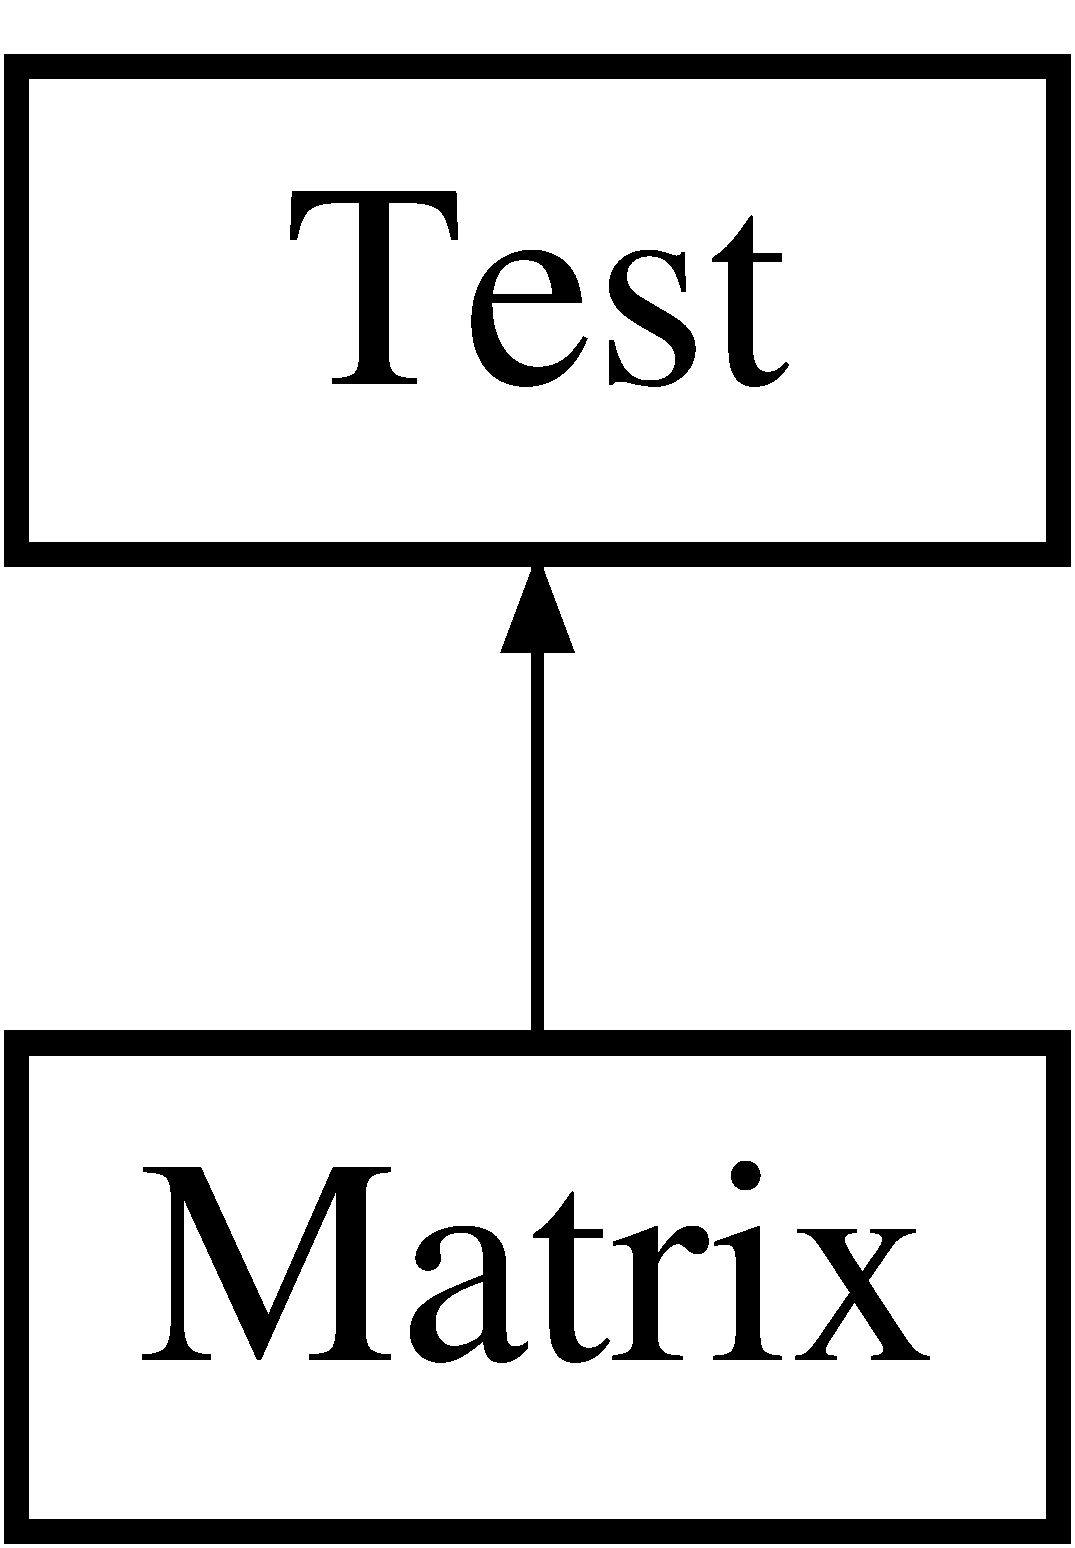
\includegraphics[height=2.000000cm]{class_matrix}
\end{center}
\end{figure}
\subsection*{Public Member Functions}
\begin{DoxyCompactItemize}
\item 
\mbox{\Hypertarget{class_matrix_af9148d60414731669dac225834d8bed4}\label{class_matrix_af9148d60414731669dac225834d8bed4}} 
{\bfseries Matrix} (\hyperlink{class_primitive_test}{Primitive\+Test}$<$ int $>$ $\ast$\+\_\+n, \hyperlink{class_primitive_test}{Primitive\+Test}$<$ int $>$ $\ast$\+\_\+m, std\+::function$<$ \hyperlink{class_test}{Test} $\ast$()$>$ \+\_\+generation\+\_\+function, std\+::string \+\_\+delimiter=\char`\"{} \char`\"{}, std\+::string \+\_\+line\+\_\+breaker=\char`\"{}\textbackslash{})
\item 
\mbox{\Hypertarget{class_matrix_a2d3097d07161be83f5a8d7f7609d57d7}\label{class_matrix_a2d3097d07161be83f5a8d7f7609d57d7}} 
{\bfseries Matrix} (\hyperlink{class_primitive_test}{Primitive\+Test}$<$ int $>$ $\ast$\+\_\+n, \hyperlink{class_primitive_test}{Primitive\+Test}$<$ int $>$ $\ast$\+\_\+m, \hyperlink{class_test}{Test} $\ast$\+\_\+example, std\+::string \+\_\+delimiter=\char`\"{} \char`\"{}, std\+::string \+\_\+line\+\_\+breaker=\char`\"{}\textbackslash{})
\item 
\mbox{\Hypertarget{class_matrix_a05fd5e85605d0c204f25c345b3a95e73}\label{class_matrix_a05fd5e85605d0c204f25c345b3a95e73}} 
{\bfseries Matrix} (\hyperlink{class_primitive_test}{Primitive\+Test}$<$ int $>$ $\ast$\+\_\+n, std\+::function$<$ \hyperlink{class_test}{Test} $\ast$()$>$ \+\_\+generation\+\_\+function, std\+::string \+\_\+delimiter=\char`\"{} \char`\"{}, std\+::string \+\_\+line\+\_\+breaker=\char`\"{}\textbackslash{})
\item 
\mbox{\Hypertarget{class_matrix_adc02dd10e346d973f7c10eedb03df3dc}\label{class_matrix_adc02dd10e346d973f7c10eedb03df3dc}} 
{\bfseries Matrix} (\hyperlink{class_primitive_test}{Primitive\+Test}$<$ int $>$ $\ast$\+\_\+n, \hyperlink{class_test}{Test} $\ast$\+\_\+example, std\+::string \+\_\+delimiter=\char`\"{} \char`\"{}, std\+::string \+\_\+line\+\_\+breaker=\char`\"{}\textbackslash{})
\item 
\mbox{\Hypertarget{class_matrix_ae0423e35c644fa22733a4333e5bbbdbd}\label{class_matrix_ae0423e35c644fa22733a4333e5bbbdbd}} 
virtual void {\bfseries Generate} ()
\item 
\mbox{\Hypertarget{class_matrix_a73e84f4b1db2fec828c81028b808510d}\label{class_matrix_a73e84f4b1db2fec828c81028b808510d}} 
virtual void {\bfseries Print} (std\+::ostream \&=std\+::cout) const
\item 
\mbox{\Hypertarget{class_matrix_aa5d036db7285113f78f23ba52e2181a3}\label{class_matrix_aa5d036db7285113f78f23ba52e2181a3}} 
void {\bfseries Print\+Size} (bool)
\item 
\mbox{\Hypertarget{class_matrix_ada8820cdc7df9cb0397496f994614df9}\label{class_matrix_ada8820cdc7df9cb0397496f994614df9}} 
std\+::pair$<$ int, int $>$ {\bfseries Size} ()
\item 
\mbox{\Hypertarget{class_matrix_a8aa21068138628b0009c8da68924b718}\label{class_matrix_a8aa21068138628b0009c8da68924b718}} 
virtual \hyperlink{class_matrix}{Matrix} $\ast$ {\bfseries Clone} () const
\item 
\mbox{\Hypertarget{class_matrix_a667c01a94f1c5e6c2f3a94ae62a27b4d}\label{class_matrix_a667c01a94f1c5e6c2f3a94ae62a27b4d}} 
std\+::vector$<$ \hyperlink{class_test}{Test} $\ast$ $>$ {\bfseries operator\mbox{[}$\,$\mbox{]}} (int i)
\end{DoxyCompactItemize}
\subsection*{Protected Attributes}
\begin{DoxyCompactItemize}
\item 
\mbox{\Hypertarget{class_matrix_a438f078e6bbcd0644a976c28b0ac3f30}\label{class_matrix_a438f078e6bbcd0644a976c28b0ac3f30}} 
std\+::function$<$ \hyperlink{class_test}{Test} $\ast$()$>$ {\bfseries generation\+\_\+function\+\_\+}
\item 
\mbox{\Hypertarget{class_matrix_a0901ceb2c484aabc0d1c3d17e7f8a486}\label{class_matrix_a0901ceb2c484aabc0d1c3d17e7f8a486}} 
\hyperlink{class_test}{Test} $\ast$ {\bfseries example\+\_\+}
\item 
\mbox{\Hypertarget{class_matrix_a3e9d1073fdbcde43ee028a6405970746}\label{class_matrix_a3e9d1073fdbcde43ee028a6405970746}} 
\hyperlink{class_primitive_test}{Primitive\+Test}$<$ int $>$ $\ast$ {\bfseries n\+\_\+}
\item 
\mbox{\Hypertarget{class_matrix_a2790a160b50a135357ae20b9fae613e6}\label{class_matrix_a2790a160b50a135357ae20b9fae613e6}} 
\hyperlink{class_primitive_test}{Primitive\+Test}$<$ int $>$ $\ast$ {\bfseries m\+\_\+}
\item 
\mbox{\Hypertarget{class_matrix_ab03d74c673757f8163e262cd521a98ae}\label{class_matrix_ab03d74c673757f8163e262cd521a98ae}} 
std\+::vector$<$ std\+::vector$<$ \hyperlink{class_test}{Test} $\ast$ $>$ $>$ {\bfseries matrix\+\_\+}
\item 
\mbox{\Hypertarget{class_matrix_a663fb05d113edfe4a05f326cdeb1177d}\label{class_matrix_a663fb05d113edfe4a05f326cdeb1177d}} 
std\+::string {\bfseries delimiter\+\_\+}
\item 
\mbox{\Hypertarget{class_matrix_a0ea53f948bd31468c744de899eb1e662}\label{class_matrix_a0ea53f948bd31468c744de899eb1e662}} 
std\+::string {\bfseries line\+\_\+breaker\+\_\+}
\item 
\mbox{\Hypertarget{class_matrix_a639e660065b416929aae3c37fa36fb27}\label{class_matrix_a639e660065b416929aae3c37fa36fb27}} 
bool {\bfseries print\+\_\+size\+\_\+}
\item 
\mbox{\Hypertarget{class_matrix_a7030785bad549a53de17ba99b9a05521}\label{class_matrix_a7030785bad549a53de17ba99b9a05521}} 
bool {\bfseries print\+\_\+size\+\_\+as\+\_\+square\+\_\+}
\end{DoxyCompactItemize}


The documentation for this class was generated from the following files\+:\begin{DoxyCompactItemize}
\item 
Matrix.\+h\item 
Matrix.\+cpp\end{DoxyCompactItemize}

\hypertarget{class_reg_ex_1_1_operation}{}\section{Reg\+Ex\+:\+:Operation Class Reference}
\label{class_reg_ex_1_1_operation}\index{Reg\+Ex\+::\+Operation@{Reg\+Ex\+::\+Operation}}
Inheritance diagram for Reg\+Ex\+:\+:Operation\+:\begin{figure}[H]
\begin{center}
\leavevmode
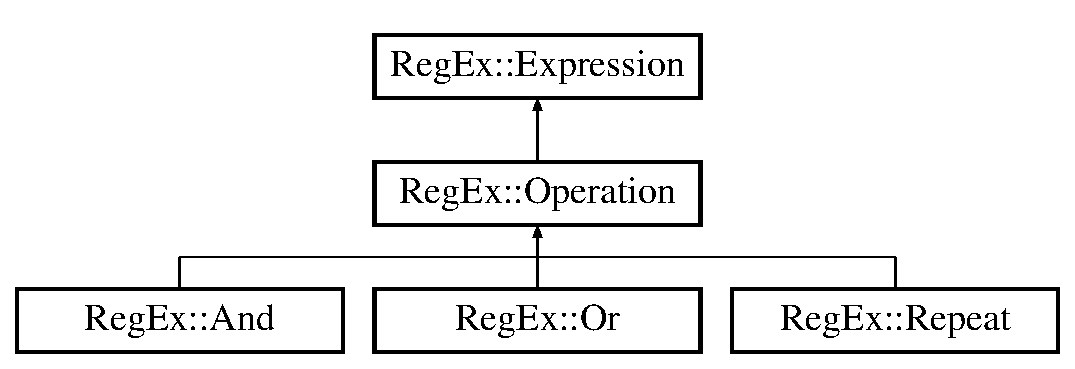
\includegraphics[height=3.000000cm]{class_reg_ex_1_1_operation}
\end{center}
\end{figure}
\subsection*{Public Member Functions}
\begin{DoxyCompactItemize}
\item 
\mbox{\Hypertarget{class_reg_ex_1_1_operation_af8c49dedc8e289586f38b6c4f5c544d2}\label{class_reg_ex_1_1_operation_af8c49dedc8e289586f38b6c4f5c544d2}} 
virtual void {\bfseries Generate} ()=0
\item 
\mbox{\Hypertarget{class_reg_ex_1_1_operation_aca61b02ac8e2bd4bdcb9c13e62b7fe85}\label{class_reg_ex_1_1_operation_aca61b02ac8e2bd4bdcb9c13e62b7fe85}} 
virtual std\+::string {\bfseries Get} ()=0
\end{DoxyCompactItemize}
\subsection*{Protected Attributes}
\begin{DoxyCompactItemize}
\item 
\mbox{\Hypertarget{class_reg_ex_1_1_operation_a2c58edc54d112abfba6b822a3f383890}\label{class_reg_ex_1_1_operation_a2c58edc54d112abfba6b822a3f383890}} 
std\+::vector$<$ \hyperlink{class_reg_ex_1_1_expression}{Expression} $\ast$ $>$ {\bfseries subexps\+\_\+}
\end{DoxyCompactItemize}


The documentation for this class was generated from the following file\+:\begin{DoxyCompactItemize}
\item 
Reg\+Ex.\+h\end{DoxyCompactItemize}

\hypertarget{class_reg_ex_1_1_or}{}\section{Reg\+Ex\+:\+:Or Class Reference}
\label{class_reg_ex_1_1_or}\index{Reg\+Ex\+::\+Or@{Reg\+Ex\+::\+Or}}
Inheritance diagram for Reg\+Ex\+:\+:Or\+:\begin{figure}[H]
\begin{center}
\leavevmode
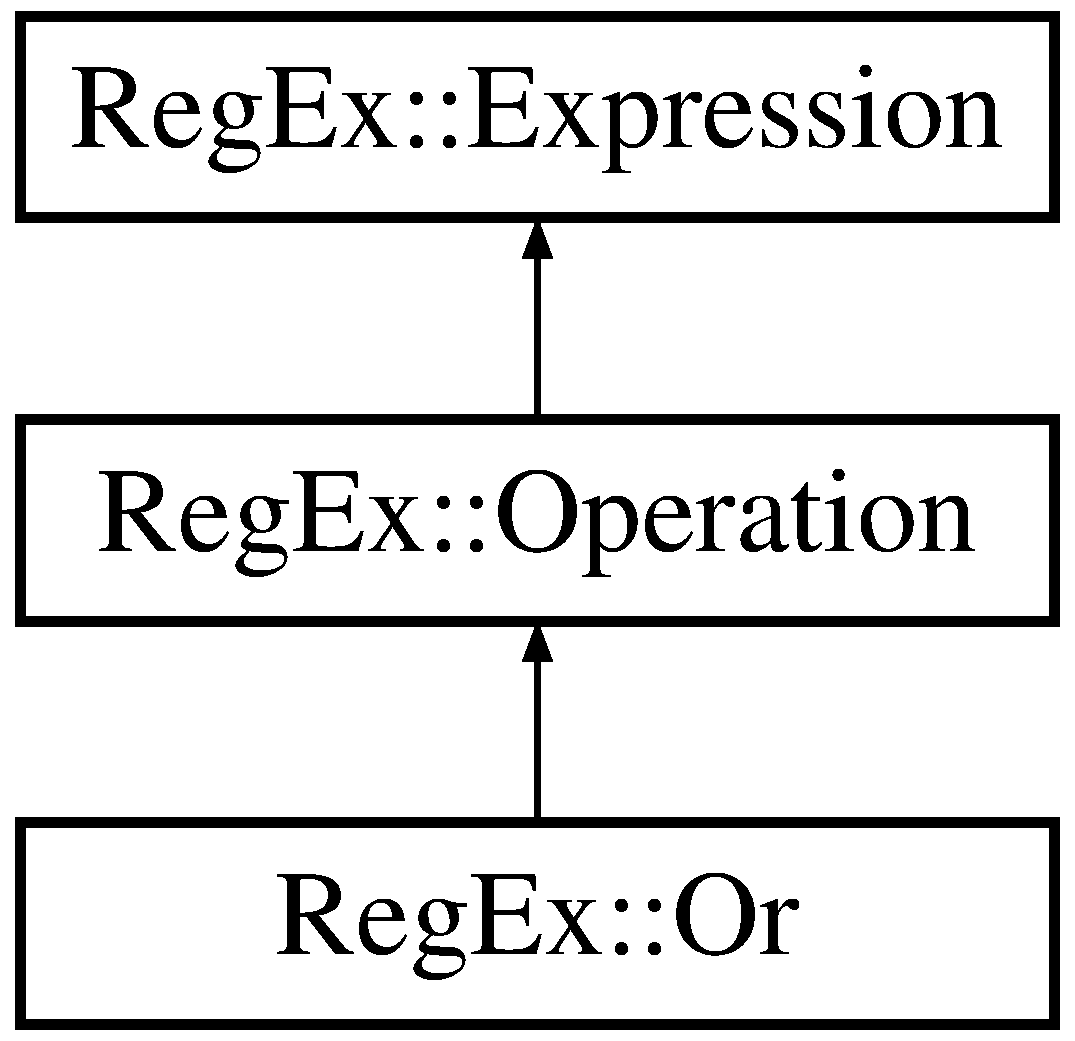
\includegraphics[height=3.000000cm]{class_reg_ex_1_1_or}
\end{center}
\end{figure}
\subsection*{Public Member Functions}
\begin{DoxyCompactItemize}
\item 
\mbox{\Hypertarget{class_reg_ex_1_1_or_a7254999b350c9f21636a10b1a4046832}\label{class_reg_ex_1_1_or_a7254999b350c9f21636a10b1a4046832}} 
void {\bfseries Add} (\hyperlink{class_reg_ex_1_1_expression}{Expression} $\ast$\+\_\+exp)
\item 
\mbox{\Hypertarget{class_reg_ex_1_1_or_a7b6fdaf356c6f252079c3472f9f63be6}\label{class_reg_ex_1_1_or_a7b6fdaf356c6f252079c3472f9f63be6}} 
virtual void {\bfseries Generate} ()
\item 
\mbox{\Hypertarget{class_reg_ex_1_1_or_a300c7c7959046826aa1e8f47f9e1a7c5}\label{class_reg_ex_1_1_or_a300c7c7959046826aa1e8f47f9e1a7c5}} 
virtual std\+::string {\bfseries Get} ()
\end{DoxyCompactItemize}
\subsection*{Protected Attributes}
\begin{DoxyCompactItemize}
\item 
\mbox{\Hypertarget{class_reg_ex_1_1_or_a62c3a11f31f6af1cc6c86063e2756b41}\label{class_reg_ex_1_1_or_a62c3a11f31f6af1cc6c86063e2756b41}} 
std\+::vector$<$ \hyperlink{class_reg_ex_1_1_expression}{Expression} $\ast$ $>$ {\bfseries subexps\+\_\+}
\item 
\mbox{\Hypertarget{class_reg_ex_1_1_or_a3ad04a1b156a610397b97832724fb2e0}\label{class_reg_ex_1_1_or_a3ad04a1b156a610397b97832724fb2e0}} 
int {\bfseries current\+\_\+element\+\_\+}
\end{DoxyCompactItemize}


The documentation for this class was generated from the following file\+:\begin{DoxyCompactItemize}
\item 
Reg\+Ex.\+h\end{DoxyCompactItemize}

\hypertarget{class_palindrome}{}\section{Palindrome Class Reference}
\label{class_palindrome}\index{Palindrome@{Palindrome}}
Inheritance diagram for Palindrome\+:\begin{figure}[H]
\begin{center}
\leavevmode
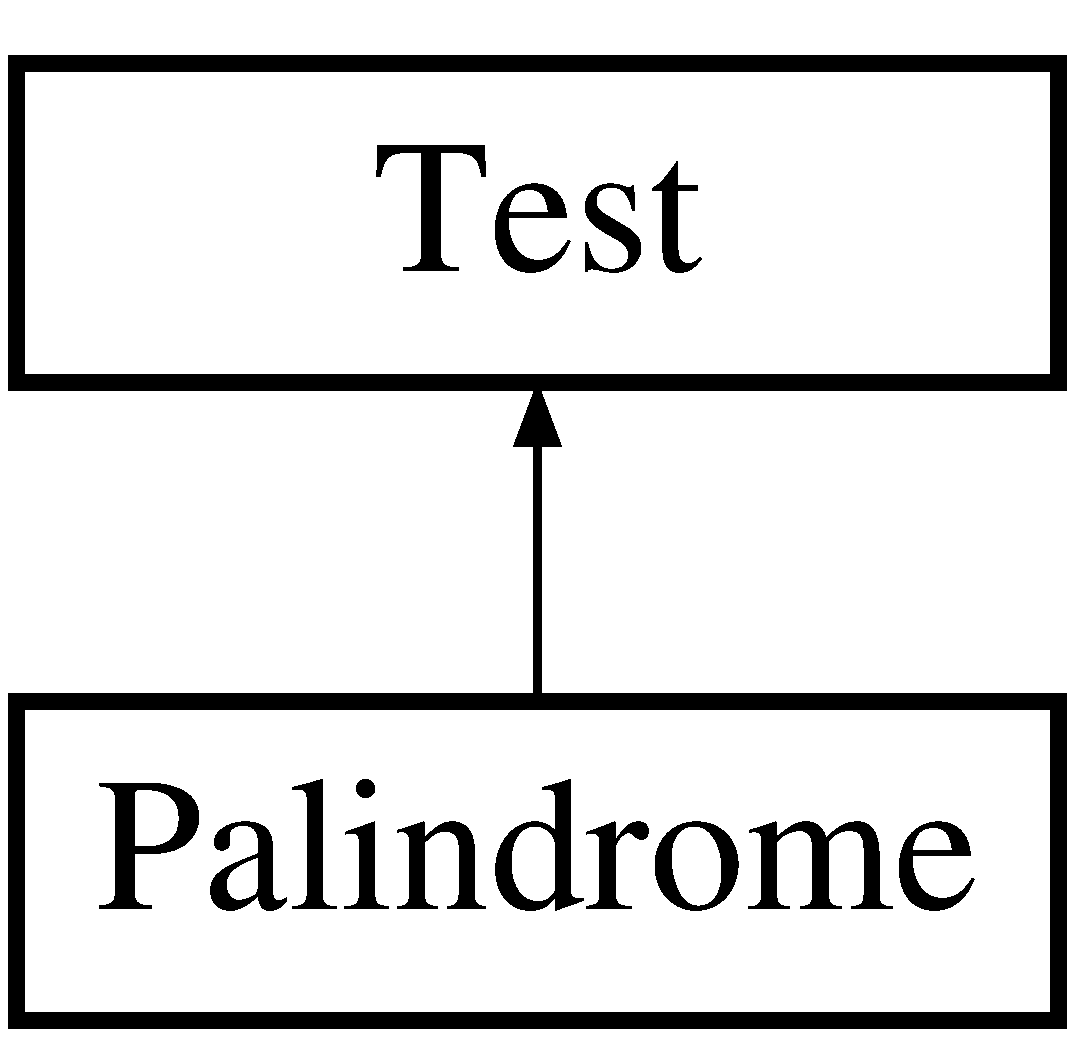
\includegraphics[height=2.000000cm]{class_palindrome}
\end{center}
\end{figure}
\subsection*{Public Member Functions}
\begin{DoxyCompactItemize}
\item 
\mbox{\Hypertarget{class_palindrome_adfc7f126cd4cd25c0fad6b280c50a3b5}\label{class_palindrome_adfc7f126cd4cd25c0fad6b280c50a3b5}} 
{\bfseries Palindrome} (\hyperlink{class_primitive_test}{Primitive\+Test}$<$ int $>$ $\ast$\+\_\+count)
\item 
\mbox{\Hypertarget{class_palindrome_a58fad4fabc60bed8450dd62d30b23862}\label{class_palindrome_a58fad4fabc60bed8450dd62d30b23862}} 
virtual void {\bfseries Generate} ()
\item 
\mbox{\Hypertarget{class_palindrome_ae526b6957989ce2d073263e5e11d0f61}\label{class_palindrome_ae526b6957989ce2d073263e5e11d0f61}} 
virtual void {\bfseries Print} (std\+::ostream \&\+\_\+out) const
\item 
\mbox{\Hypertarget{class_palindrome_abacf8a157ffb07913fa1300b02245634}\label{class_palindrome_abacf8a157ffb07913fa1300b02245634}} 
virtual \hyperlink{class_test}{Test} $\ast$ {\bfseries Clone} () const
\end{DoxyCompactItemize}
\subsection*{Additional Inherited Members}


The documentation for this class was generated from the following file\+:\begin{DoxyCompactItemize}
\item 
Source.\+cpp\end{DoxyCompactItemize}

\hypertarget{class_primitive_test}{}\section{Primitive\+Test$<$ T $>$ Class Template Reference}
\label{class_primitive_test}\index{Primitive\+Test$<$ T $>$@{Primitive\+Test$<$ T $>$}}
Inheritance diagram for Primitive\+Test$<$ T $>$\+:\begin{figure}[H]
\begin{center}
\leavevmode
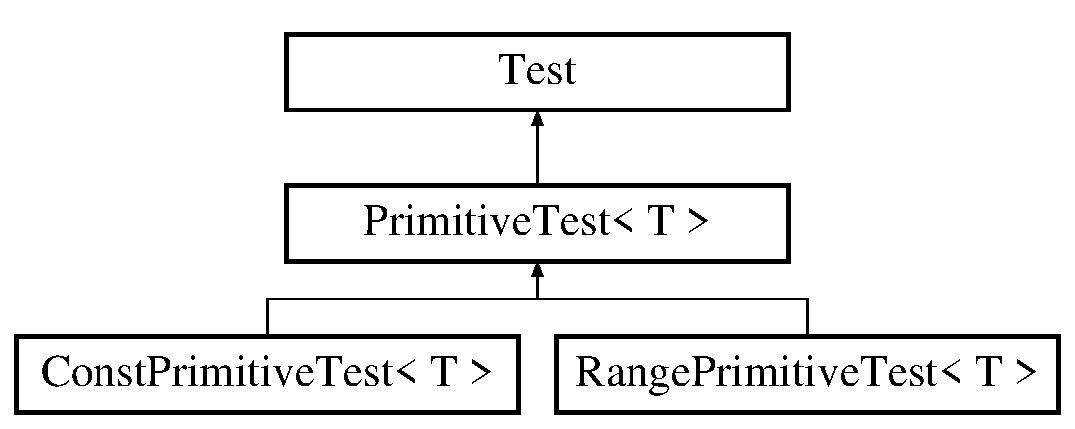
\includegraphics[height=3.000000cm]{class_primitive_test}
\end{center}
\end{figure}
\subsection*{Public Member Functions}
\begin{DoxyCompactItemize}
\item 
\mbox{\Hypertarget{class_primitive_test_a330ccae6cebf4cd196a1087838b3bb3f}\label{class_primitive_test_a330ccae6cebf4cd196a1087838b3bb3f}} 
virtual T {\bfseries Get} ()=0
\item 
\mbox{\Hypertarget{class_primitive_test_a83aa7e6514500d5a470d9a437088bb1d}\label{class_primitive_test_a83aa7e6514500d5a470d9a437088bb1d}} 
virtual void {\bfseries Generate} ()=0
\item 
\mbox{\Hypertarget{class_primitive_test_a7f510e857162432281fa6fed458bfd5f}\label{class_primitive_test_a7f510e857162432281fa6fed458bfd5f}} 
virtual void {\bfseries Print} (std\+::ostream \&=std\+::cout) const =0
\item 
\mbox{\Hypertarget{class_primitive_test_ac4efd25f85ac1c6d50c7e7b9c3b6e86e}\label{class_primitive_test_ac4efd25f85ac1c6d50c7e7b9c3b6e86e}} 
virtual \hyperlink{class_primitive_test}{Primitive\+Test} $\ast$ {\bfseries Clone} () const =0
\end{DoxyCompactItemize}
\subsection*{Additional Inherited Members}


The documentation for this class was generated from the following file\+:\begin{DoxyCompactItemize}
\item 
Primitive\+Test.\+h\end{DoxyCompactItemize}

\hypertarget{class_quadrilateral}{}\section{Quadrilateral Class Reference}
\label{class_quadrilateral}\index{Quadrilateral@{Quadrilateral}}
Inheritance diagram for Quadrilateral\+:\begin{figure}[H]
\begin{center}
\leavevmode
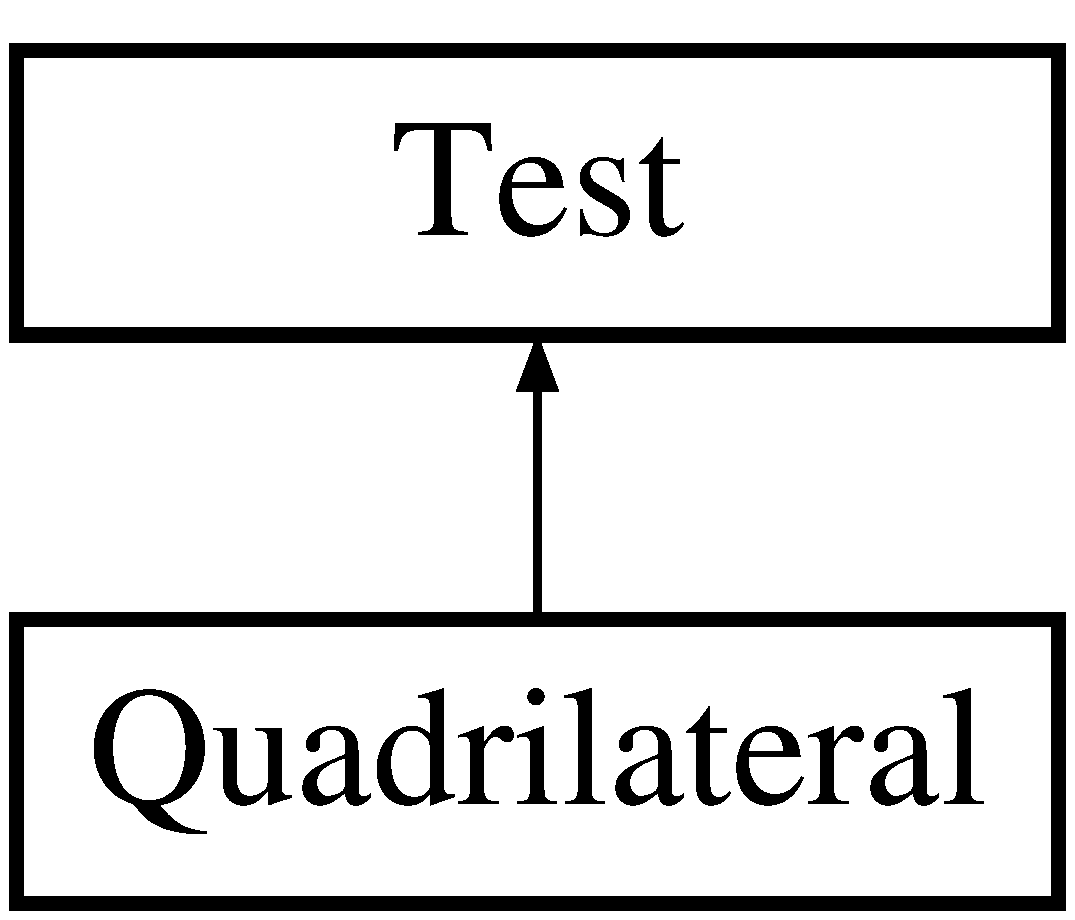
\includegraphics[height=2.000000cm]{class_quadrilateral}
\end{center}
\end{figure}
\subsection*{Public Member Functions}
\begin{DoxyCompactItemize}
\item 
\mbox{\Hypertarget{class_quadrilateral_aaa2c98ed785ae526a760e411808d19d4}\label{class_quadrilateral_aaa2c98ed785ae526a760e411808d19d4}} 
virtual void {\bfseries Generate} ()
\item 
\mbox{\Hypertarget{class_quadrilateral_a8cd7b99d0f1790e97bc90aecba0f52c1}\label{class_quadrilateral_a8cd7b99d0f1790e97bc90aecba0f52c1}} 
virtual void {\bfseries Print} (std\+::ostream \&\+\_\+out) const
\item 
\mbox{\Hypertarget{class_quadrilateral_aa68850ecd4e782c1fb452ae954858b5c}\label{class_quadrilateral_aa68850ecd4e782c1fb452ae954858b5c}} 
virtual \hyperlink{class_test}{Test} $\ast$ {\bfseries Clone} () const
\end{DoxyCompactItemize}
\subsection*{Additional Inherited Members}


The documentation for this class was generated from the following file\+:\begin{DoxyCompactItemize}
\item 
Source.\+cpp\end{DoxyCompactItemize}

\hypertarget{class_random_test_set}{}\section{Random\+Test\+Set Class Reference}
\label{class_random_test_set}\index{Random\+Test\+Set@{Random\+Test\+Set}}
Inheritance diagram for Random\+Test\+Set\+:\begin{figure}[H]
\begin{center}
\leavevmode
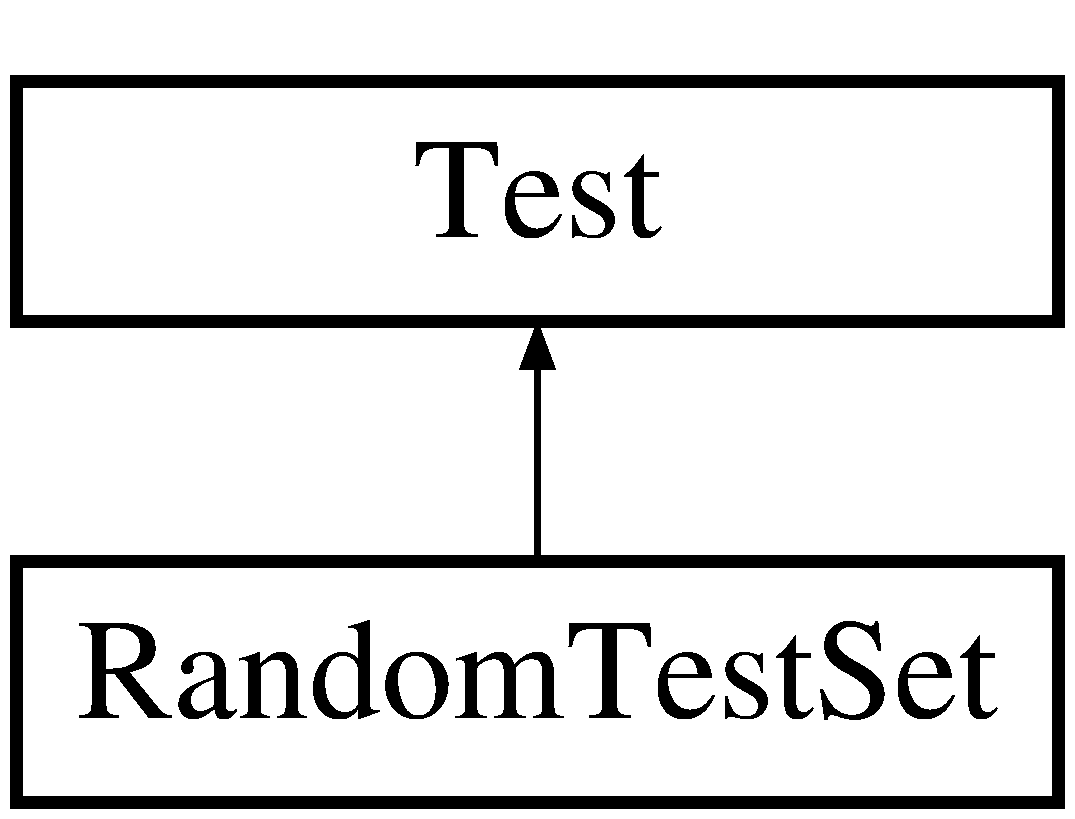
\includegraphics[height=2.000000cm]{class_random_test_set}
\end{center}
\end{figure}
\subsection*{Public Member Functions}
\begin{DoxyCompactItemize}
\item 
\mbox{\Hypertarget{class_random_test_set_a9857bd26593f8c9619946437670e8508}\label{class_random_test_set_a9857bd26593f8c9619946437670e8508}} 
virtual \hyperlink{class_random_test_set}{Random\+Test\+Set} $\ast$ {\bfseries Add} (\hyperlink{class_test}{Test} $\ast$)
\item 
\mbox{\Hypertarget{class_random_test_set_aa112670e8e1096950d064d273fe0813b}\label{class_random_test_set_aa112670e8e1096950d064d273fe0813b}} 
virtual \hyperlink{class_test}{Test} $\ast$ {\bfseries Get} ()
\item 
\mbox{\Hypertarget{class_random_test_set_a8ae5ba47a55c8aa4b12d045315e43a7f}\label{class_random_test_set_a8ae5ba47a55c8aa4b12d045315e43a7f}} 
virtual void {\bfseries Generate} ()
\item 
\mbox{\Hypertarget{class_random_test_set_a50dea8180a7ac0f2e7336f21b88b7f70}\label{class_random_test_set_a50dea8180a7ac0f2e7336f21b88b7f70}} 
virtual void {\bfseries Print} (std\+::ostream \&=std\+::cout) const
\item 
\mbox{\Hypertarget{class_random_test_set_a2a90e27b75bf2896131a9922c4afb2ed}\label{class_random_test_set_a2a90e27b75bf2896131a9922c4afb2ed}} 
virtual \hyperlink{class_random_test_set}{Random\+Test\+Set} $\ast$ {\bfseries Clone} () const
\end{DoxyCompactItemize}
\subsection*{Additional Inherited Members}


The documentation for this class was generated from the following files\+:\begin{DoxyCompactItemize}
\item 
Random\+Test\+Set.\+h\item 
Random\+Test\+Set.\+cpp\end{DoxyCompactItemize}

\hypertarget{class_range}{}\section{Range$<$ T $>$ Class Template Reference}
\label{class_range}\index{Range$<$ T $>$@{Range$<$ T $>$}}
Inheritance diagram for Range$<$ T $>$\+:\begin{figure}[H]
\begin{center}
\leavevmode
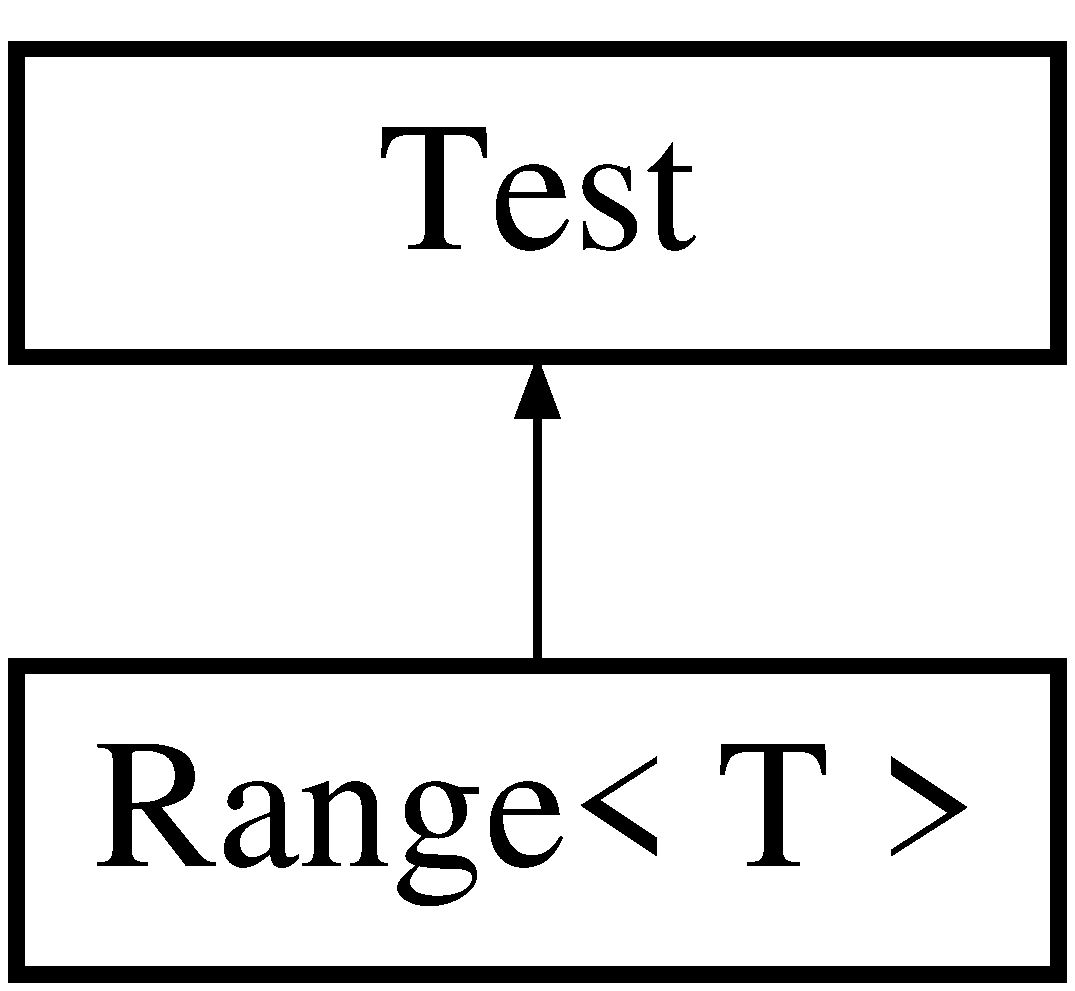
\includegraphics[height=2.000000cm]{class_range}
\end{center}
\end{figure}
\subsection*{Public Member Functions}
\begin{DoxyCompactItemize}
\item 
\mbox{\Hypertarget{class_range_a32cb63626f447ec44fac820ebe16b2d1}\label{class_range_a32cb63626f447ec44fac820ebe16b2d1}} 
{\bfseries Range} (\hyperlink{class_primitive_test}{Primitive\+Test}$<$ T $>$ $\ast$\+\_\+begin, \hyperlink{class_primitive_test}{Primitive\+Test}$<$ T $>$ $\ast$\+\_\+end)
\item 
\mbox{\Hypertarget{class_range_aadfc9764842da72211e5309484327d92}\label{class_range_aadfc9764842da72211e5309484327d92}} 
T {\bfseries Get} ()
\item 
\mbox{\Hypertarget{class_range_a2609e897d13111a4b1bc499c0ef08f0c}\label{class_range_a2609e897d13111a4b1bc499c0ef08f0c}} 
\hyperlink{class_range}{Range} $\ast$ {\bfseries Clone} () const
\item 
\mbox{\Hypertarget{class_range_a8c90569fec87e93b9f00ba87b60dbbdf}\label{class_range_a8c90569fec87e93b9f00ba87b60dbbdf}} 
virtual void {\bfseries Generate} ()
\item 
\mbox{\Hypertarget{class_range_a00c9138fb65efccb1f8d5156e067dc47}\label{class_range_a00c9138fb65efccb1f8d5156e067dc47}} 
virtual void {\bfseries Print} (std\+::ostream \&\+\_\+out) const
\item 
\mbox{\Hypertarget{class_range_a64badfcbc1a69b9dc4e2210dd3af3d5c}\label{class_range_a64badfcbc1a69b9dc4e2210dd3af3d5c}} 
void {\bfseries Range\+Validation} ()
\item 
\mbox{\Hypertarget{class_range_a60733afafbde307d7f237acc51088e67}\label{class_range_a60733afafbde307d7f237acc51088e67}} 
\hyperlink{class_range}{Range}$<$ T $>$ \& {\bfseries operator=} (T \+\_\+current\+\_\+value)
\item 
\mbox{\Hypertarget{class_range_a06b5093d33e6e7d5a6d3a7f94f744c8a}\label{class_range_a06b5093d33e6e7d5a6d3a7f94f744c8a}} 
{\footnotesize template$<$$>$ }\\long long {\bfseries Get} ()
\item 
\mbox{\Hypertarget{class_range_a05a289b5408cb3dac5f3b4c2c487a2c3}\label{class_range_a05a289b5408cb3dac5f3b4c2c487a2c3}} 
{\footnotesize template$<$$>$ }\\int {\bfseries Get} ()
\item 
\mbox{\Hypertarget{class_range_a7461e74f69c79c8b96a938f0f81a33c3}\label{class_range_a7461e74f69c79c8b96a938f0f81a33c3}} 
{\footnotesize template$<$$>$ }\\double {\bfseries Get} ()
\item 
\mbox{\Hypertarget{class_range_a7bd69d54a6135d371484e1e46ad408e9}\label{class_range_a7bd69d54a6135d371484e1e46ad408e9}} 
{\footnotesize template$<$$>$ }\\char {\bfseries Get} ()
\end{DoxyCompactItemize}
\subsection*{Protected Attributes}
\begin{DoxyCompactItemize}
\item 
\mbox{\Hypertarget{class_range_ad0c538b07b483db50faaf728cf3fd72b}\label{class_range_ad0c538b07b483db50faaf728cf3fd72b}} 
\hyperlink{class_primitive_test}{Primitive\+Test}$<$ T $>$ $\ast$ {\bfseries begin\+\_\+}
\item 
\mbox{\Hypertarget{class_range_a5c057e464e0dc930245b123369c2c1ea}\label{class_range_a5c057e464e0dc930245b123369c2c1ea}} 
\hyperlink{class_primitive_test}{Primitive\+Test}$<$ T $>$ $\ast$ {\bfseries end\+\_\+}
\end{DoxyCompactItemize}
\subsection*{Friends}
\begin{DoxyCompactItemize}
\item 
\mbox{\Hypertarget{class_range_a13a243c96bb300c01fe9842da0e9dfda}\label{class_range_a13a243c96bb300c01fe9842da0e9dfda}} 
\hyperlink{class_range}{Range}$<$ T $>$ \& {\bfseries operator$>$} (\hyperlink{class_range}{Range}$<$ T $>$ \&\+\_\+range, T \+\_\+lower)
\item 
\mbox{\Hypertarget{class_range_a69fd53e9c8f9af069f9ab99be90b87a0}\label{class_range_a69fd53e9c8f9af069f9ab99be90b87a0}} 
\hyperlink{class_range}{Range}$<$ T $>$ \& {\bfseries operator$<$} (T \+\_\+lower, \hyperlink{class_range}{Range}$<$ T $>$ \&\+\_\+range)
\item 
\mbox{\Hypertarget{class_range_a76bb66c47ced37fe31ff78c8ac227890}\label{class_range_a76bb66c47ced37fe31ff78c8ac227890}} 
\hyperlink{class_range}{Range}$<$ T $>$ \& {\bfseries operator$>$} (T \+\_\+greater, \hyperlink{class_range}{Range}$<$ T $>$ \&\+\_\+range)
\item 
\mbox{\Hypertarget{class_range_a633d4f94f44b3bb09a3214ce91ace3ae}\label{class_range_a633d4f94f44b3bb09a3214ce91ace3ae}} 
\hyperlink{class_range}{Range}$<$ T $>$ \& {\bfseries operator$<$} (\hyperlink{class_range}{Range}$<$ T $>$ \&\+\_\+range, T \+\_\+greater)
\end{DoxyCompactItemize}


The documentation for this class was generated from the following file\+:\begin{DoxyCompactItemize}
\item 
Range.\+h\end{DoxyCompactItemize}

\hypertarget{class_range_primitive_test}{}\section{Range\+Primitive\+Test$<$ T $>$ Class Template Reference}
\label{class_range_primitive_test}\index{Range\+Primitive\+Test$<$ T $>$@{Range\+Primitive\+Test$<$ T $>$}}
Inheritance diagram for Range\+Primitive\+Test$<$ T $>$\+:\begin{figure}[H]
\begin{center}
\leavevmode
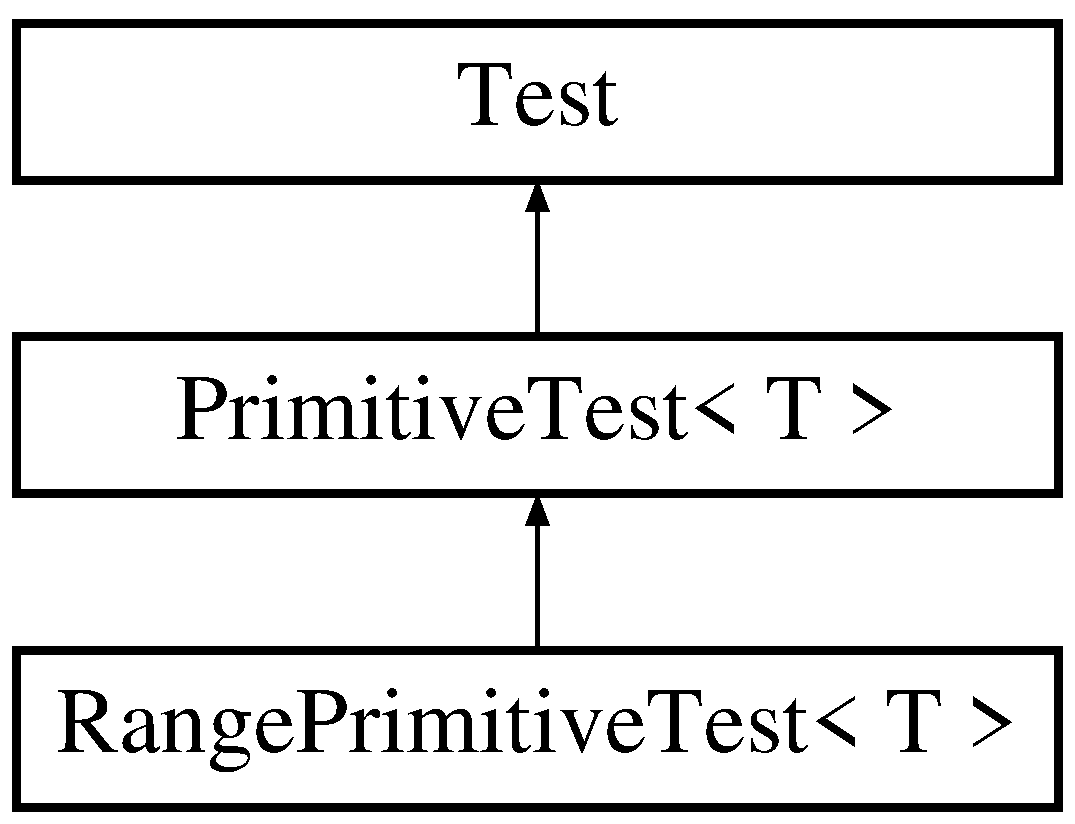
\includegraphics[height=3.000000cm]{class_range_primitive_test}
\end{center}
\end{figure}
\subsection*{Public Member Functions}
\begin{DoxyCompactItemize}
\item 
\mbox{\Hypertarget{class_range_primitive_test_aa6661f7649f14fb09b1f2dd61e181f75}\label{class_range_primitive_test_aa6661f7649f14fb09b1f2dd61e181f75}} 
{\bfseries Range\+Primitive\+Test} (\hyperlink{class_range}{Range}$<$ T $>$ $\ast$\+\_\+range)
\item 
\mbox{\Hypertarget{class_range_primitive_test_a5d6683558e9057c056a5a8229b7fca5f}\label{class_range_primitive_test_a5d6683558e9057c056a5a8229b7fca5f}} 
{\bfseries Range\+Primitive\+Test} (int \+\_\+start=0, int \+\_\+end=0)
\item 
\mbox{\Hypertarget{class_range_primitive_test_af0d7709c56a1a3e06e70572a09b3c921}\label{class_range_primitive_test_af0d7709c56a1a3e06e70572a09b3c921}} 
virtual T {\bfseries Get} ()
\item 
\mbox{\Hypertarget{class_range_primitive_test_afcca64a473c09008aadbe42367ac71ba}\label{class_range_primitive_test_afcca64a473c09008aadbe42367ac71ba}} 
virtual void {\bfseries Generate} ()
\item 
\mbox{\Hypertarget{class_range_primitive_test_a01ef34f0ffee1bb38f2ae4ce8754cb25}\label{class_range_primitive_test_a01ef34f0ffee1bb38f2ae4ce8754cb25}} 
virtual void {\bfseries Print} (std\+::ostream \&\+\_\+out=std\+::cout) const
\item 
\mbox{\Hypertarget{class_range_primitive_test_a9539da245360c39d3da0a1ce8df56f6d}\label{class_range_primitive_test_a9539da245360c39d3da0a1ce8df56f6d}} 
virtual \hyperlink{class_range_primitive_test}{Range\+Primitive\+Test} $\ast$ {\bfseries Clone} () const
\end{DoxyCompactItemize}
\subsection*{Friends}
\begin{DoxyCompactItemize}
\item 
\mbox{\Hypertarget{class_range_primitive_test_adc4b5e0edfdc33b7847e865fa9a0156f}\label{class_range_primitive_test_adc4b5e0edfdc33b7847e865fa9a0156f}} 
\hyperlink{class_range_primitive_test}{Range\+Primitive\+Test}$<$ T $>$ \& {\bfseries operator$>$} (\hyperlink{class_range_primitive_test}{Range\+Primitive\+Test}$<$ T $>$ \&\+\_\+rpt, T \+\_\+lower)
\item 
\mbox{\Hypertarget{class_range_primitive_test_aa8ef9c7ab9cddca084117fbd68f51e43}\label{class_range_primitive_test_aa8ef9c7ab9cddca084117fbd68f51e43}} 
\hyperlink{class_range_primitive_test}{Range\+Primitive\+Test}$<$ T $>$ \& {\bfseries operator$<$} (T \+\_\+lower, \hyperlink{class_range_primitive_test}{Range\+Primitive\+Test}$<$ T $>$ \&\+\_\+rpt)
\item 
\mbox{\Hypertarget{class_range_primitive_test_a86324f8ee9d7a253b83c767017aaec5c}\label{class_range_primitive_test_a86324f8ee9d7a253b83c767017aaec5c}} 
\hyperlink{class_range_primitive_test}{Range\+Primitive\+Test}$<$ T $>$ \& {\bfseries operator$>$} (T \+\_\+greater, \hyperlink{class_range_primitive_test}{Range\+Primitive\+Test}$<$ T $>$ \&\+\_\+rpt)
\item 
\mbox{\Hypertarget{class_range_primitive_test_a60d8ecdb646db1900aa59cc3600eb8cb}\label{class_range_primitive_test_a60d8ecdb646db1900aa59cc3600eb8cb}} 
\hyperlink{class_range_primitive_test}{Range\+Primitive\+Test}$<$ T $>$ \& {\bfseries operator$<$} (\hyperlink{class_range_primitive_test}{Range\+Primitive\+Test}$<$ T $>$ \&\+\_\+rpt, T \+\_\+greater)
\end{DoxyCompactItemize}
\subsection*{Additional Inherited Members}


The documentation for this class was generated from the following file\+:\begin{DoxyCompactItemize}
\item 
Range\+Primitive\+Test.\+h\end{DoxyCompactItemize}

\hypertarget{class_reg_ex}{}\section{Reg\+Ex Class Reference}
\label{class_reg_ex}\index{Reg\+Ex@{Reg\+Ex}}
Inheritance diagram for Reg\+Ex\+:\begin{figure}[H]
\begin{center}
\leavevmode
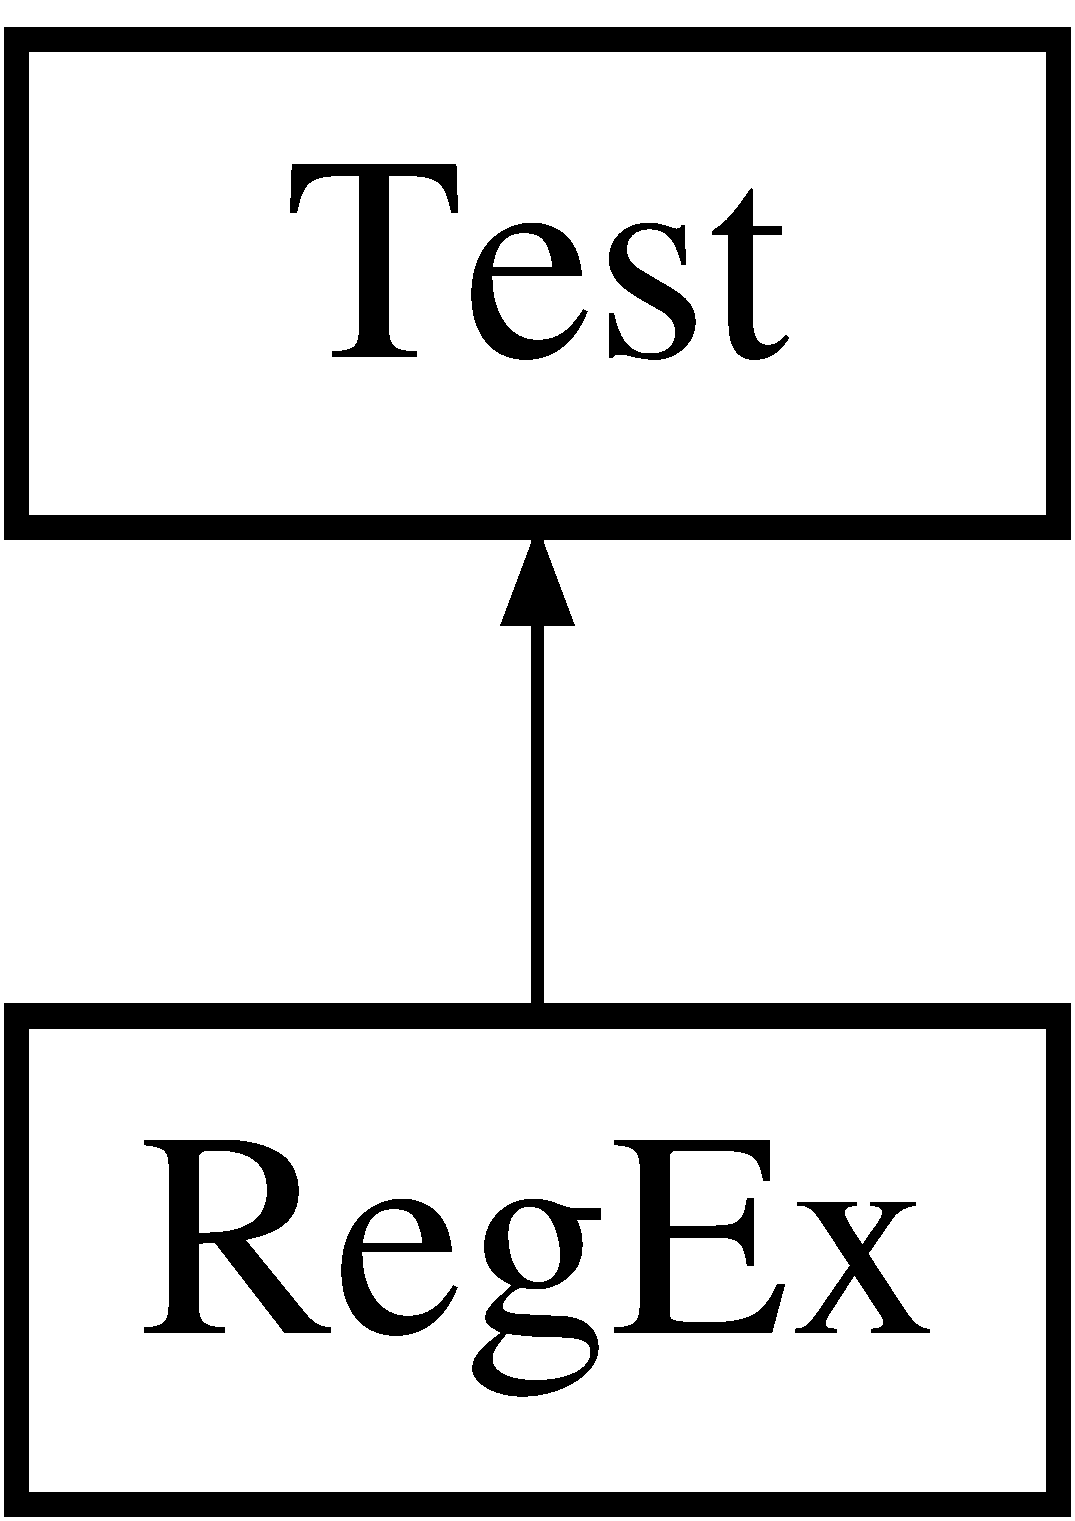
\includegraphics[height=2.000000cm]{class_reg_ex}
\end{center}
\end{figure}
\subsection*{Classes}
\begin{DoxyCompactItemize}
\item 
class \hyperlink{class_reg_ex_1_1_and}{And}
\item 
class \hyperlink{class_reg_ex_1_1_expression}{Expression}
\item 
class \hyperlink{class_reg_ex_1_1_operation}{Operation}
\item 
class \hyperlink{class_reg_ex_1_1_or}{Or}
\item 
class \hyperlink{class_reg_ex_1_1_repeat}{Repeat}
\item 
class \hyperlink{class_reg_ex_1_1_terminal}{Terminal}
\end{DoxyCompactItemize}
\subsection*{Public Member Functions}
\begin{DoxyCompactItemize}
\item 
\mbox{\Hypertarget{class_reg_ex_a7b5051ee106f62bc682bdb6060ebbda3}\label{class_reg_ex_a7b5051ee106f62bc682bdb6060ebbda3}} 
{\bfseries Reg\+Ex} (const std\+::string \&, int=1000)
\item 
\mbox{\Hypertarget{class_reg_ex_afd916615e5ad551dc487489be89bee1e}\label{class_reg_ex_afd916615e5ad551dc487489be89bee1e}} 
virtual void {\bfseries Generate} ()
\item 
\mbox{\Hypertarget{class_reg_ex_a049ff6ccf8e7ce6fe03d08dc37318867}\label{class_reg_ex_a049ff6ccf8e7ce6fe03d08dc37318867}} 
virtual std\+::string {\bfseries Get} ()
\item 
\mbox{\Hypertarget{class_reg_ex_a6ace1d67d2958a15f0d9b88b11fe330c}\label{class_reg_ex_a6ace1d67d2958a15f0d9b88b11fe330c}} 
virtual void {\bfseries Print} (std\+::ostream \&=std\+::cout) const
\item 
\mbox{\Hypertarget{class_reg_ex_a3b10fe7fa64453168762bd06d2af748d}\label{class_reg_ex_a3b10fe7fa64453168762bd06d2af748d}} 
virtual void {\bfseries Max\+Lenght} (int \+\_\+max\+\_\+size)
\item 
\mbox{\Hypertarget{class_reg_ex_a1c31c684cfa651d5954c0f8ec054d844}\label{class_reg_ex_a1c31c684cfa651d5954c0f8ec054d844}} 
virtual \hyperlink{class_reg_ex}{Reg\+Ex} $\ast$ {\bfseries Clone} () const
\end{DoxyCompactItemize}
\subsection*{Protected Attributes}
\begin{DoxyCompactItemize}
\item 
\mbox{\Hypertarget{class_reg_ex_af928b29986284f40a2859c2953084ea2}\label{class_reg_ex_af928b29986284f40a2859c2953084ea2}} 
\hyperlink{class_reg_ex_1_1_expression}{Expression} $\ast$ {\bfseries regex\+\_\+exp}
\item 
\mbox{\Hypertarget{class_reg_ex_af11c2a0136d196abea09421b70bd6309}\label{class_reg_ex_af11c2a0136d196abea09421b70bd6309}} 
std\+::string {\bfseries regex\+\_\+}
\item 
\mbox{\Hypertarget{class_reg_ex_a04ecf5608b4ec9509ab0b9392b32ba1f}\label{class_reg_ex_a04ecf5608b4ec9509ab0b9392b32ba1f}} 
std\+::string {\bfseries current\+\_\+string\+\_\+}
\item 
\mbox{\Hypertarget{class_reg_ex_a215472f429e78fab0fee7c6deac05928}\label{class_reg_ex_a215472f429e78fab0fee7c6deac05928}} 
int {\bfseries max\+\_\+lenght\+\_\+}
\end{DoxyCompactItemize}


The documentation for this class was generated from the following files\+:\begin{DoxyCompactItemize}
\item 
Reg\+Ex.\+h\item 
Reg\+Ex.\+cpp\end{DoxyCompactItemize}

\hypertarget{class_reg_ex_1_1_repeat}{}\section{Reg\+Ex\+:\+:Repeat Class Reference}
\label{class_reg_ex_1_1_repeat}\index{Reg\+Ex\+::\+Repeat@{Reg\+Ex\+::\+Repeat}}
Inheritance diagram for Reg\+Ex\+:\+:Repeat\+:\begin{figure}[H]
\begin{center}
\leavevmode
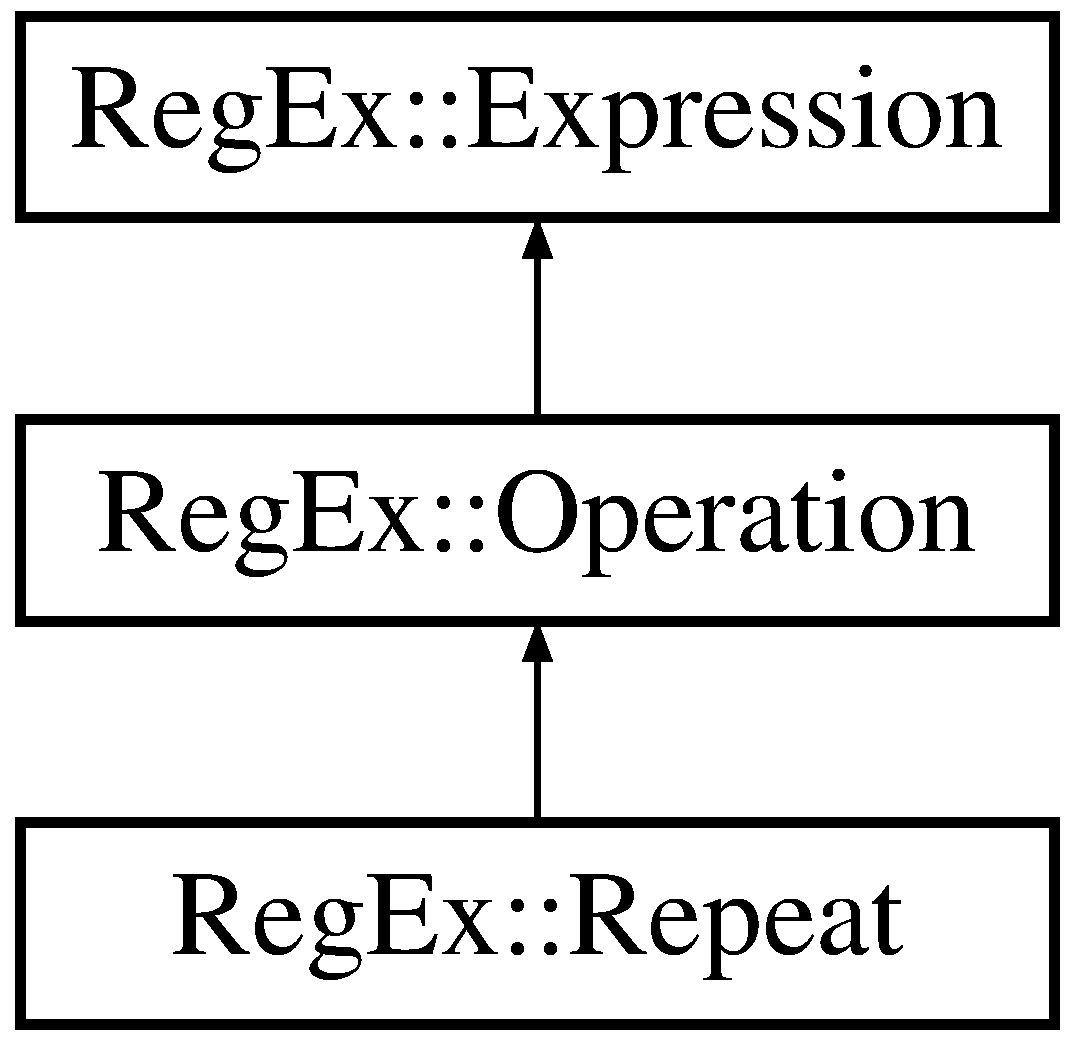
\includegraphics[height=3.000000cm]{class_reg_ex_1_1_repeat}
\end{center}
\end{figure}
\subsection*{Public Member Functions}
\begin{DoxyCompactItemize}
\item 
\mbox{\Hypertarget{class_reg_ex_1_1_repeat_a6889fa0984149563767aa76380621994}\label{class_reg_ex_1_1_repeat_a6889fa0984149563767aa76380621994}} 
{\bfseries Repeat} (\hyperlink{class_reg_ex_1_1_expression}{Expression} $\ast$\+\_\+exp, \hyperlink{class_primitive_test}{Primitive\+Test}$<$ int $>$ $\ast$\+\_\+count)
\item 
\mbox{\Hypertarget{class_reg_ex_1_1_repeat_aa7f9520f00c1e283da55996f97fa0691}\label{class_reg_ex_1_1_repeat_aa7f9520f00c1e283da55996f97fa0691}} 
virtual void {\bfseries Generate} ()
\item 
\mbox{\Hypertarget{class_reg_ex_1_1_repeat_a8de75c8cc3dd1e781aaed6810a7d9cc3}\label{class_reg_ex_1_1_repeat_a8de75c8cc3dd1e781aaed6810a7d9cc3}} 
virtual std\+::string {\bfseries Get} ()
\end{DoxyCompactItemize}
\subsection*{Protected Attributes}
\begin{DoxyCompactItemize}
\item 
\mbox{\Hypertarget{class_reg_ex_1_1_repeat_a68b7bb97e81f625484b995b97660b9f5}\label{class_reg_ex_1_1_repeat_a68b7bb97e81f625484b995b97660b9f5}} 
\hyperlink{class_reg_ex_1_1_expression}{Expression} $\ast$ {\bfseries exp\+\_\+}
\item 
\mbox{\Hypertarget{class_reg_ex_1_1_repeat_a8b286ece3065c515d7d43f402affdb48}\label{class_reg_ex_1_1_repeat_a8b286ece3065c515d7d43f402affdb48}} 
\hyperlink{class_primitive_test}{Primitive\+Test}$<$ int $>$ $\ast$ {\bfseries count\+\_\+}
\end{DoxyCompactItemize}


The documentation for this class was generated from the following file\+:\begin{DoxyCompactItemize}
\item 
Reg\+Ex.\+h\end{DoxyCompactItemize}

\hypertarget{class_r_n_g}{}\section{R\+NG Class Reference}
\label{class_r_n_g}\index{R\+NG@{R\+NG}}
\subsection*{Static Public Member Functions}
\begin{DoxyCompactItemize}
\item 
\mbox{\Hypertarget{class_r_n_g_a427cbd39e534df7411d93ba48c4076ca}\label{class_r_n_g_a427cbd39e534df7411d93ba48c4076ca}} 
static long long {\bfseries Rand} ()
\item 
\mbox{\Hypertarget{class_r_n_g_aaab24bbee351a128618027d201cabdfb}\label{class_r_n_g_aaab24bbee351a128618027d201cabdfb}} 
static void {\bfseries Random\+Function} (std\+::function$<$ int()$>$ \+\_\+rng\+\_\+function)
\item 
\mbox{\Hypertarget{class_r_n_g_a1a3d5ecdf4b60266eba3b7d375920135}\label{class_r_n_g_a1a3d5ecdf4b60266eba3b7d375920135}} 
static void {\bfseries Random\+Seed} (unsigned int \+\_\+seed)
\end{DoxyCompactItemize}


The documentation for this class was generated from the following files\+:\begin{DoxyCompactItemize}
\item 
Utils.\+h\item 
Utils.\+cpp\end{DoxyCompactItemize}

\hypertarget{class_reg_ex_1_1_terminal}{}\section{Reg\+Ex\+:\+:Terminal Class Reference}
\label{class_reg_ex_1_1_terminal}\index{Reg\+Ex\+::\+Terminal@{Reg\+Ex\+::\+Terminal}}
Inheritance diagram for Reg\+Ex\+:\+:Terminal\+:\begin{figure}[H]
\begin{center}
\leavevmode
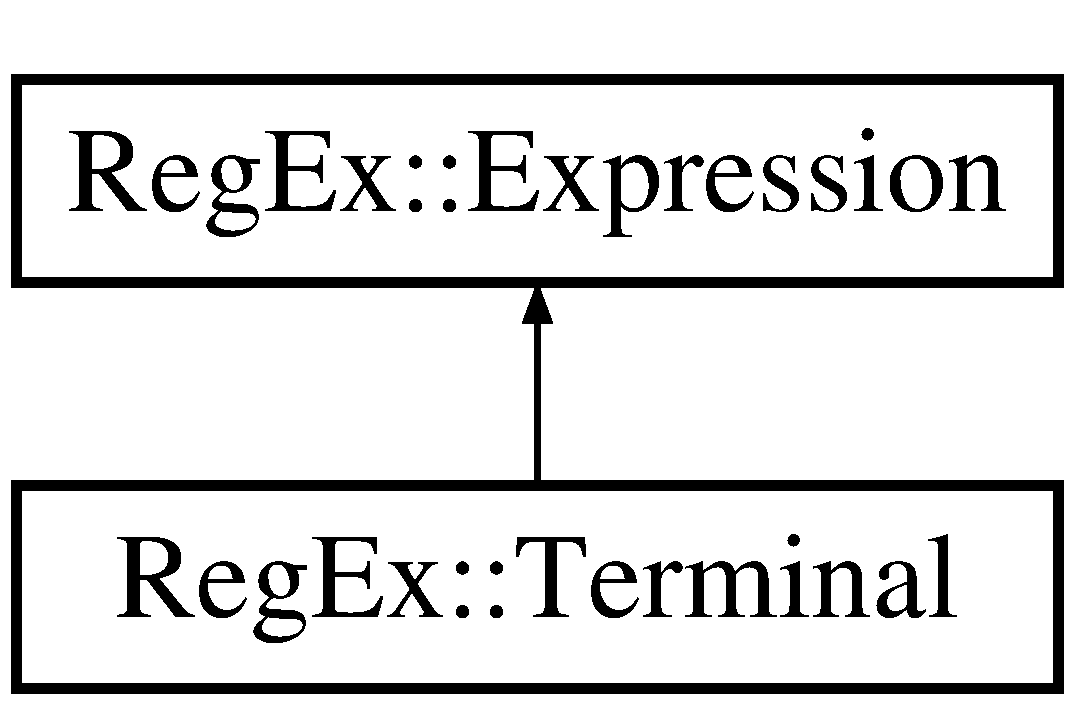
\includegraphics[height=2.000000cm]{class_reg_ex_1_1_terminal}
\end{center}
\end{figure}
\subsection*{Public Member Functions}
\begin{DoxyCompactItemize}
\item 
\mbox{\Hypertarget{class_reg_ex_1_1_terminal_a006d1b7c4c76d5c4780242d374ab7231}\label{class_reg_ex_1_1_terminal_a006d1b7c4c76d5c4780242d374ab7231}} 
{\bfseries Terminal} (char c)
\item 
\mbox{\Hypertarget{class_reg_ex_1_1_terminal_ad028ff321058247c2a8dc221fea5ccd6}\label{class_reg_ex_1_1_terminal_ad028ff321058247c2a8dc221fea5ccd6}} 
{\bfseries Terminal} (const std\+::string \&\+\_\+regex)
\item 
\mbox{\Hypertarget{class_reg_ex_1_1_terminal_aa2fe782395367b60378cde6fa8ce1ffa}\label{class_reg_ex_1_1_terminal_aa2fe782395367b60378cde6fa8ce1ffa}} 
void {\bfseries Generate} ()
\item 
\mbox{\Hypertarget{class_reg_ex_1_1_terminal_ac29198abae509962e6f41203a1bb8caf}\label{class_reg_ex_1_1_terminal_ac29198abae509962e6f41203a1bb8caf}} 
std\+::string {\bfseries Get} ()
\end{DoxyCompactItemize}


The documentation for this class was generated from the following file\+:\begin{DoxyCompactItemize}
\item 
Reg\+Ex.\+h\end{DoxyCompactItemize}

\hypertarget{class_test}{}\section{Test Class Reference}
\label{class_test}\index{Test@{Test}}
Inheritance diagram for Test\+:\begin{figure}[H]
\begin{center}
\leavevmode
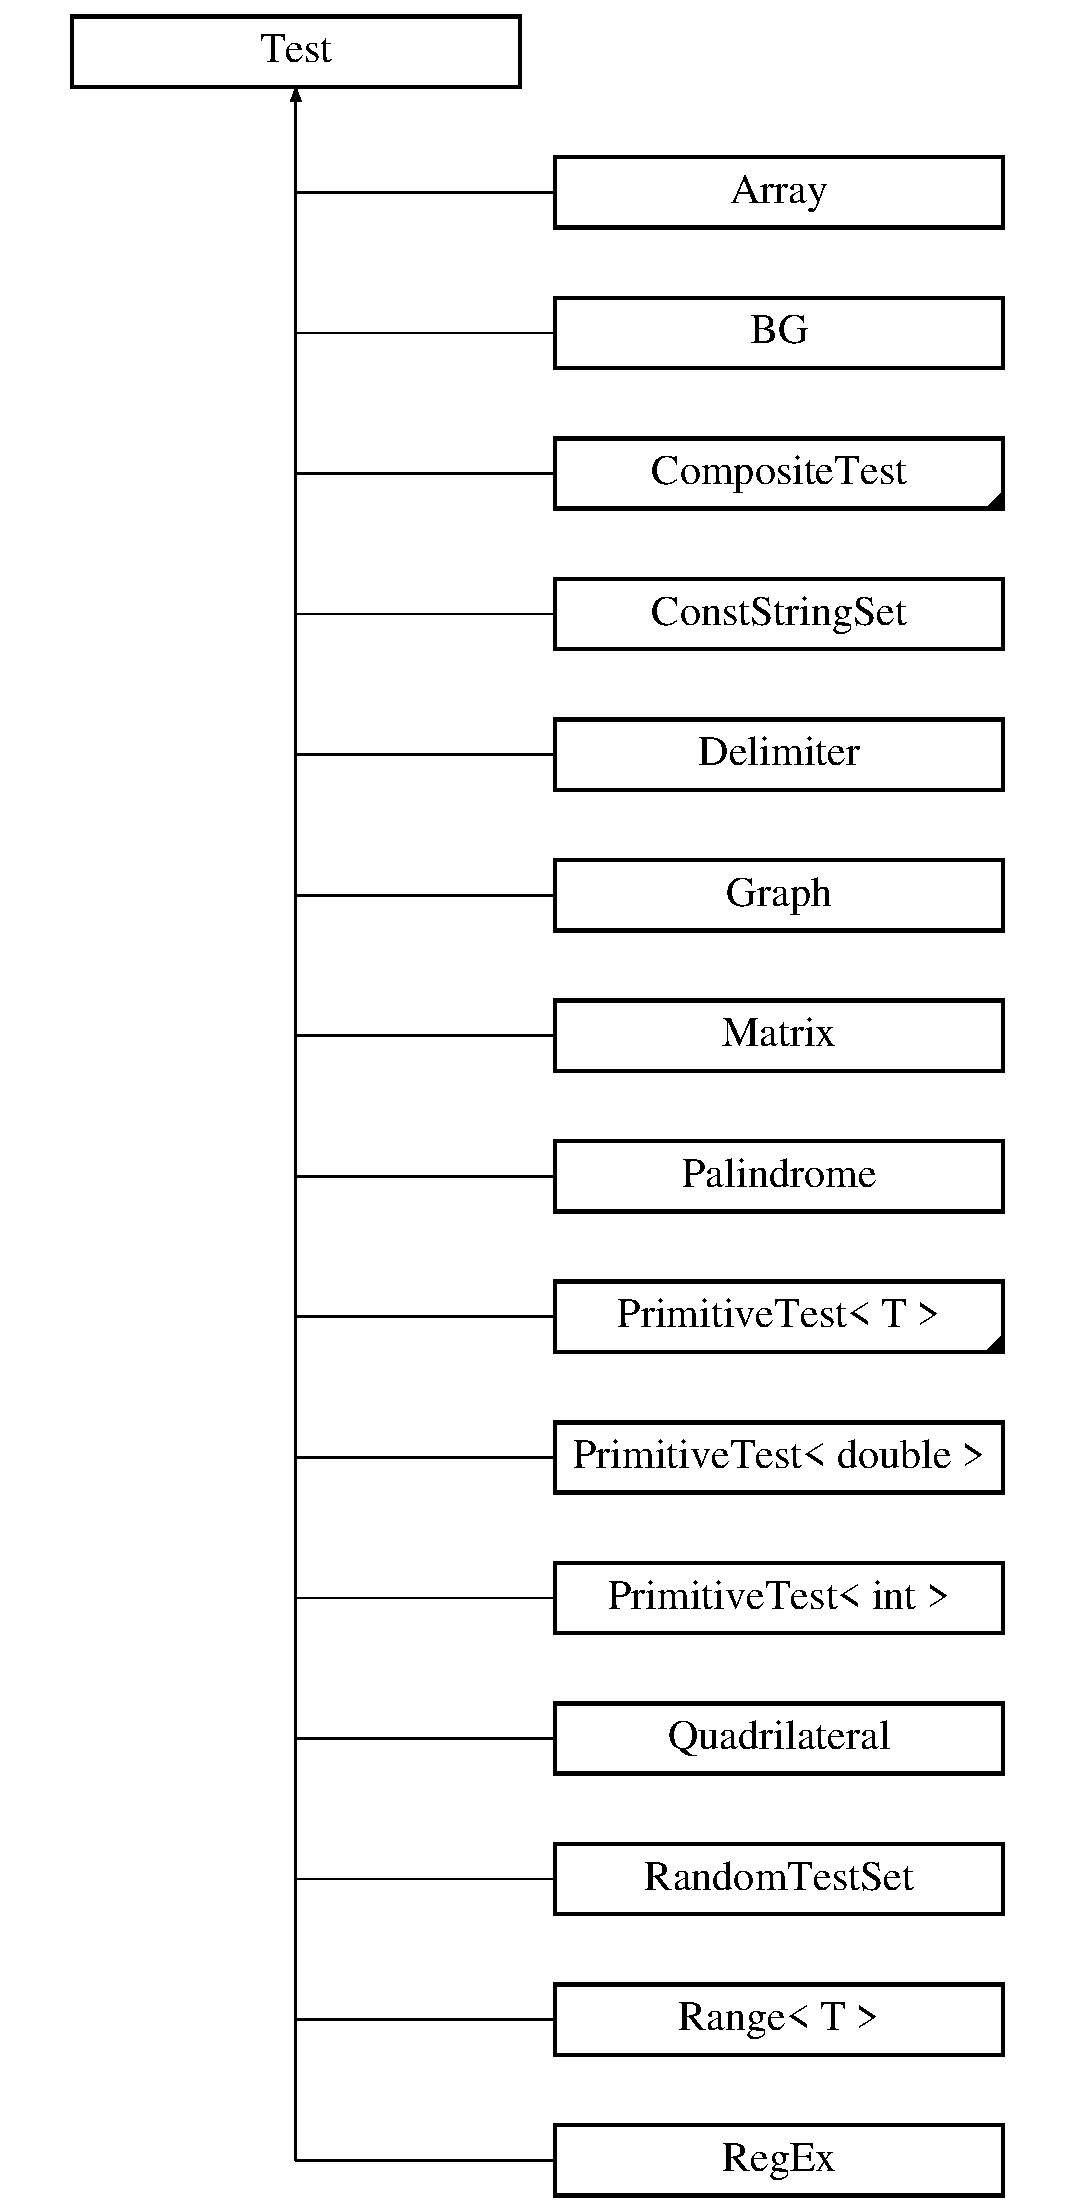
\includegraphics[height=12.000000cm]{class_test}
\end{center}
\end{figure}
\subsection*{Public Member Functions}
\begin{DoxyCompactItemize}
\item 
\mbox{\Hypertarget{class_test_ae733fa615b80df74a8eead13eff258bd}\label{class_test_ae733fa615b80df74a8eead13eff258bd}} 
virtual void {\bfseries Generate} ()=0
\item 
\mbox{\Hypertarget{class_test_a0f822839f807872aa12de4163638f1d8}\label{class_test_a0f822839f807872aa12de4163638f1d8}} 
virtual void {\bfseries Print} (std\+::ostream \&=std\+::cout) const =0
\item 
\mbox{\Hypertarget{class_test_a859196a50bc6fb1e5153c38ecbef0ab1}\label{class_test_a859196a50bc6fb1e5153c38ecbef0ab1}} 
virtual \hyperlink{class_test}{Test} $\ast$ {\bfseries Clone} () const =0
\item 
\mbox{\Hypertarget{class_test_a9dee176f10107d101a682a6b1bc60d10}\label{class_test_a9dee176f10107d101a682a6b1bc60d10}} 
virtual \hyperlink{class_test}{Test} $\ast$ {\bfseries Add} (\hyperlink{class_test}{Test} $\ast$)
\item 
\mbox{\Hypertarget{class_test_a6246397d122b42ed7ea3af9aa15221b2}\label{class_test_a6246397d122b42ed7ea3af9aa15221b2}} 
virtual void {\bfseries Add\+Delete\+Responsibility} (\hyperlink{class_test}{Test} $\ast$\+\_\+object)
\end{DoxyCompactItemize}
\subsection*{Protected Attributes}
\begin{DoxyCompactItemize}
\item 
\mbox{\Hypertarget{class_test_aa0c74215e7ebe83f150fd976df2a2f0c}\label{class_test_aa0c74215e7ebe83f150fd976df2a2f0c}} 
bool {\bfseries test\+\_\+generated\+\_\+}
\item 
\mbox{\Hypertarget{class_test_a6d134f96b13a6d97991731bfeb60d086}\label{class_test_a6d134f96b13a6d97991731bfeb60d086}} 
std\+::vector$<$ \hyperlink{class_test}{Test} $\ast$ $>$ {\bfseries objects\+\_\+with\+\_\+delete\+\_\+responsibility\+\_\+}
\end{DoxyCompactItemize}


The documentation for this class was generated from the following file\+:\begin{DoxyCompactItemize}
\item 
Test.\+h\end{DoxyCompactItemize}

\hypertarget{class_test_creator}{}\section{Test\+Creator Class Reference}
\label{class_test_creator}\index{Test\+Creator@{Test\+Creator}}
\subsection*{Public Member Functions}
\begin{DoxyCompactItemize}
\item 
\mbox{\Hypertarget{class_test_creator_a42e7313422d75e9142bc8f53024c78e8}\label{class_test_creator_a42e7313422d75e9142bc8f53024c78e8}} 
{\bfseries Test\+Creator} (\hyperlink{class_test}{Test} $\ast$\+\_\+test, int \+\_\+times, std\+::string \+\_\+path, int \+\_\+number\+\_\+of\+\_\+threads=1, std\+::string \+\_\+file\+\_\+name\+\_\+prefix=std\+::string(), std\+::string \+\_\+extension=\char`\"{}.txt\char`\"{}, int \+\_\+start\+\_\+from=0)
\item 
\mbox{\Hypertarget{class_test_creator_aca1be1f7abe92337cb78b9fcb39a7887}\label{class_test_creator_aca1be1f7abe92337cb78b9fcb39a7887}} 
void {\bfseries Make} ()
\end{DoxyCompactItemize}
\subsection*{Protected Member Functions}
\begin{DoxyCompactItemize}
\item 
\mbox{\Hypertarget{class_test_creator_a7008308857ea20fca5f1178519a1ef62}\label{class_test_creator_a7008308857ea20fca5f1178519a1ef62}} 
void {\bfseries Test\+Generating} (int interval\+\_\+start, int interval\+\_\+end)
\end{DoxyCompactItemize}
\subsection*{Protected Attributes}
\begin{DoxyCompactItemize}
\item 
\mbox{\Hypertarget{class_test_creator_a4f8fecd5a07c62d4f2fcdfe7139a5ccf}\label{class_test_creator_a4f8fecd5a07c62d4f2fcdfe7139a5ccf}} 
\hyperlink{class_test}{Test} $\ast$ {\bfseries test\+\_\+}
\item 
\mbox{\Hypertarget{class_test_creator_ab2ac1e5aa9682b89d2ffd2d4b9657e09}\label{class_test_creator_ab2ac1e5aa9682b89d2ffd2d4b9657e09}} 
std\+::string {\bfseries path\+\_\+}
\item 
\mbox{\Hypertarget{class_test_creator_a9bbb73aa599bdd2455ea3acd6ae422ac}\label{class_test_creator_a9bbb73aa599bdd2455ea3acd6ae422ac}} 
int {\bfseries times\+\_\+}
\item 
\mbox{\Hypertarget{class_test_creator_a4e56773a1a47da7d416e3258b0a9a11f}\label{class_test_creator_a4e56773a1a47da7d416e3258b0a9a11f}} 
int {\bfseries number\+\_\+of\+\_\+threads\+\_\+}
\item 
\mbox{\Hypertarget{class_test_creator_ac1c7262d75e3b547efdd774514a4f8e3}\label{class_test_creator_ac1c7262d75e3b547efdd774514a4f8e3}} 
std\+::string {\bfseries file\+\_\+name\+\_\+prefix\+\_\+}
\item 
\mbox{\Hypertarget{class_test_creator_a76c471dd1f4bdb04c1fd71c779f2cbab}\label{class_test_creator_a76c471dd1f4bdb04c1fd71c779f2cbab}} 
std\+::string {\bfseries extension\+\_\+}
\item 
\mbox{\Hypertarget{class_test_creator_ac4db98afb823de08926f31b54218d736}\label{class_test_creator_ac4db98afb823de08926f31b54218d736}} 
int {\bfseries start\+\_\+from\+\_\+}
\end{DoxyCompactItemize}


The documentation for this class was generated from the following file\+:\begin{DoxyCompactItemize}
\item 
Test\+Creator.\+h\end{DoxyCompactItemize}

%--- End generated contents ---

% Index
\backmatter
\newpage
\phantomsection
\clearemptydoublepage
\addcontentsline{toc}{chapter}{Index}
\printindex

\end{document}
